\renewcommand*{\thefootnote}{\arabic{footnote}}

\mbox{}\\
\vspace{8cm}

\section{The global impact of microbial pathogens} \label{sec:_intro_global_impact}

The \ac{GBD} 2019 study reported that microbial pathogens are responsible for more than 400 million years of life lost annually across the globe, a higher burden than either cancer or cardiovascular disease \citep{vos_global_2020}. 
In particular, lower respiratory infections, diarrhoeal diseases, HIV/AIDS and tuberculosis were amongst the five leading causes of global total years of life lost. 
More recently, the COVID-19 pandemic, declared as such by the \ac{WHO} on 11 March 2020 after the emergence and global spread of the \ac{SARS-CoV-2}, has caused more than 5 million deaths worldwide \citep{ritchie_coronavirus_2020}, making it one of the deadliest pandemics in history.
Coronavirus has been responsible for three of the 18 major pandemics recorded throughout modern history \citep{piret_pandemics_2021}, all occurring after the year 2000.
\textit{Yersinia pestis}, responsible for three plague pandemics, \textit{Vibrio cholerae}, with seven cholera pandemics, and Influenza A virus, the causal agent of five flu pandemics, are responsible for the remaining, Influenza being the only other pathogen with a pandemic registered after the year 2000. 
Recent decades have also witnessed the emergence of additional virulent pathogens, including the Ebola virus, West Nile virus, Dengue virus and Zika virus, particularly in lower-income countries.

In addition to the emergence of virulent pathogens, the rise of \ac{AMR} poses a major threat to human health around the world. 
Besides tuberculosis, the global priority due to being the most common and lethal airborne \ac{AMR} disease worldwide today, responsible for 250,000 deaths each year, it includes 12 groups of pathogens in three priority categories. 

\begin{figure*}[h!]
\centering
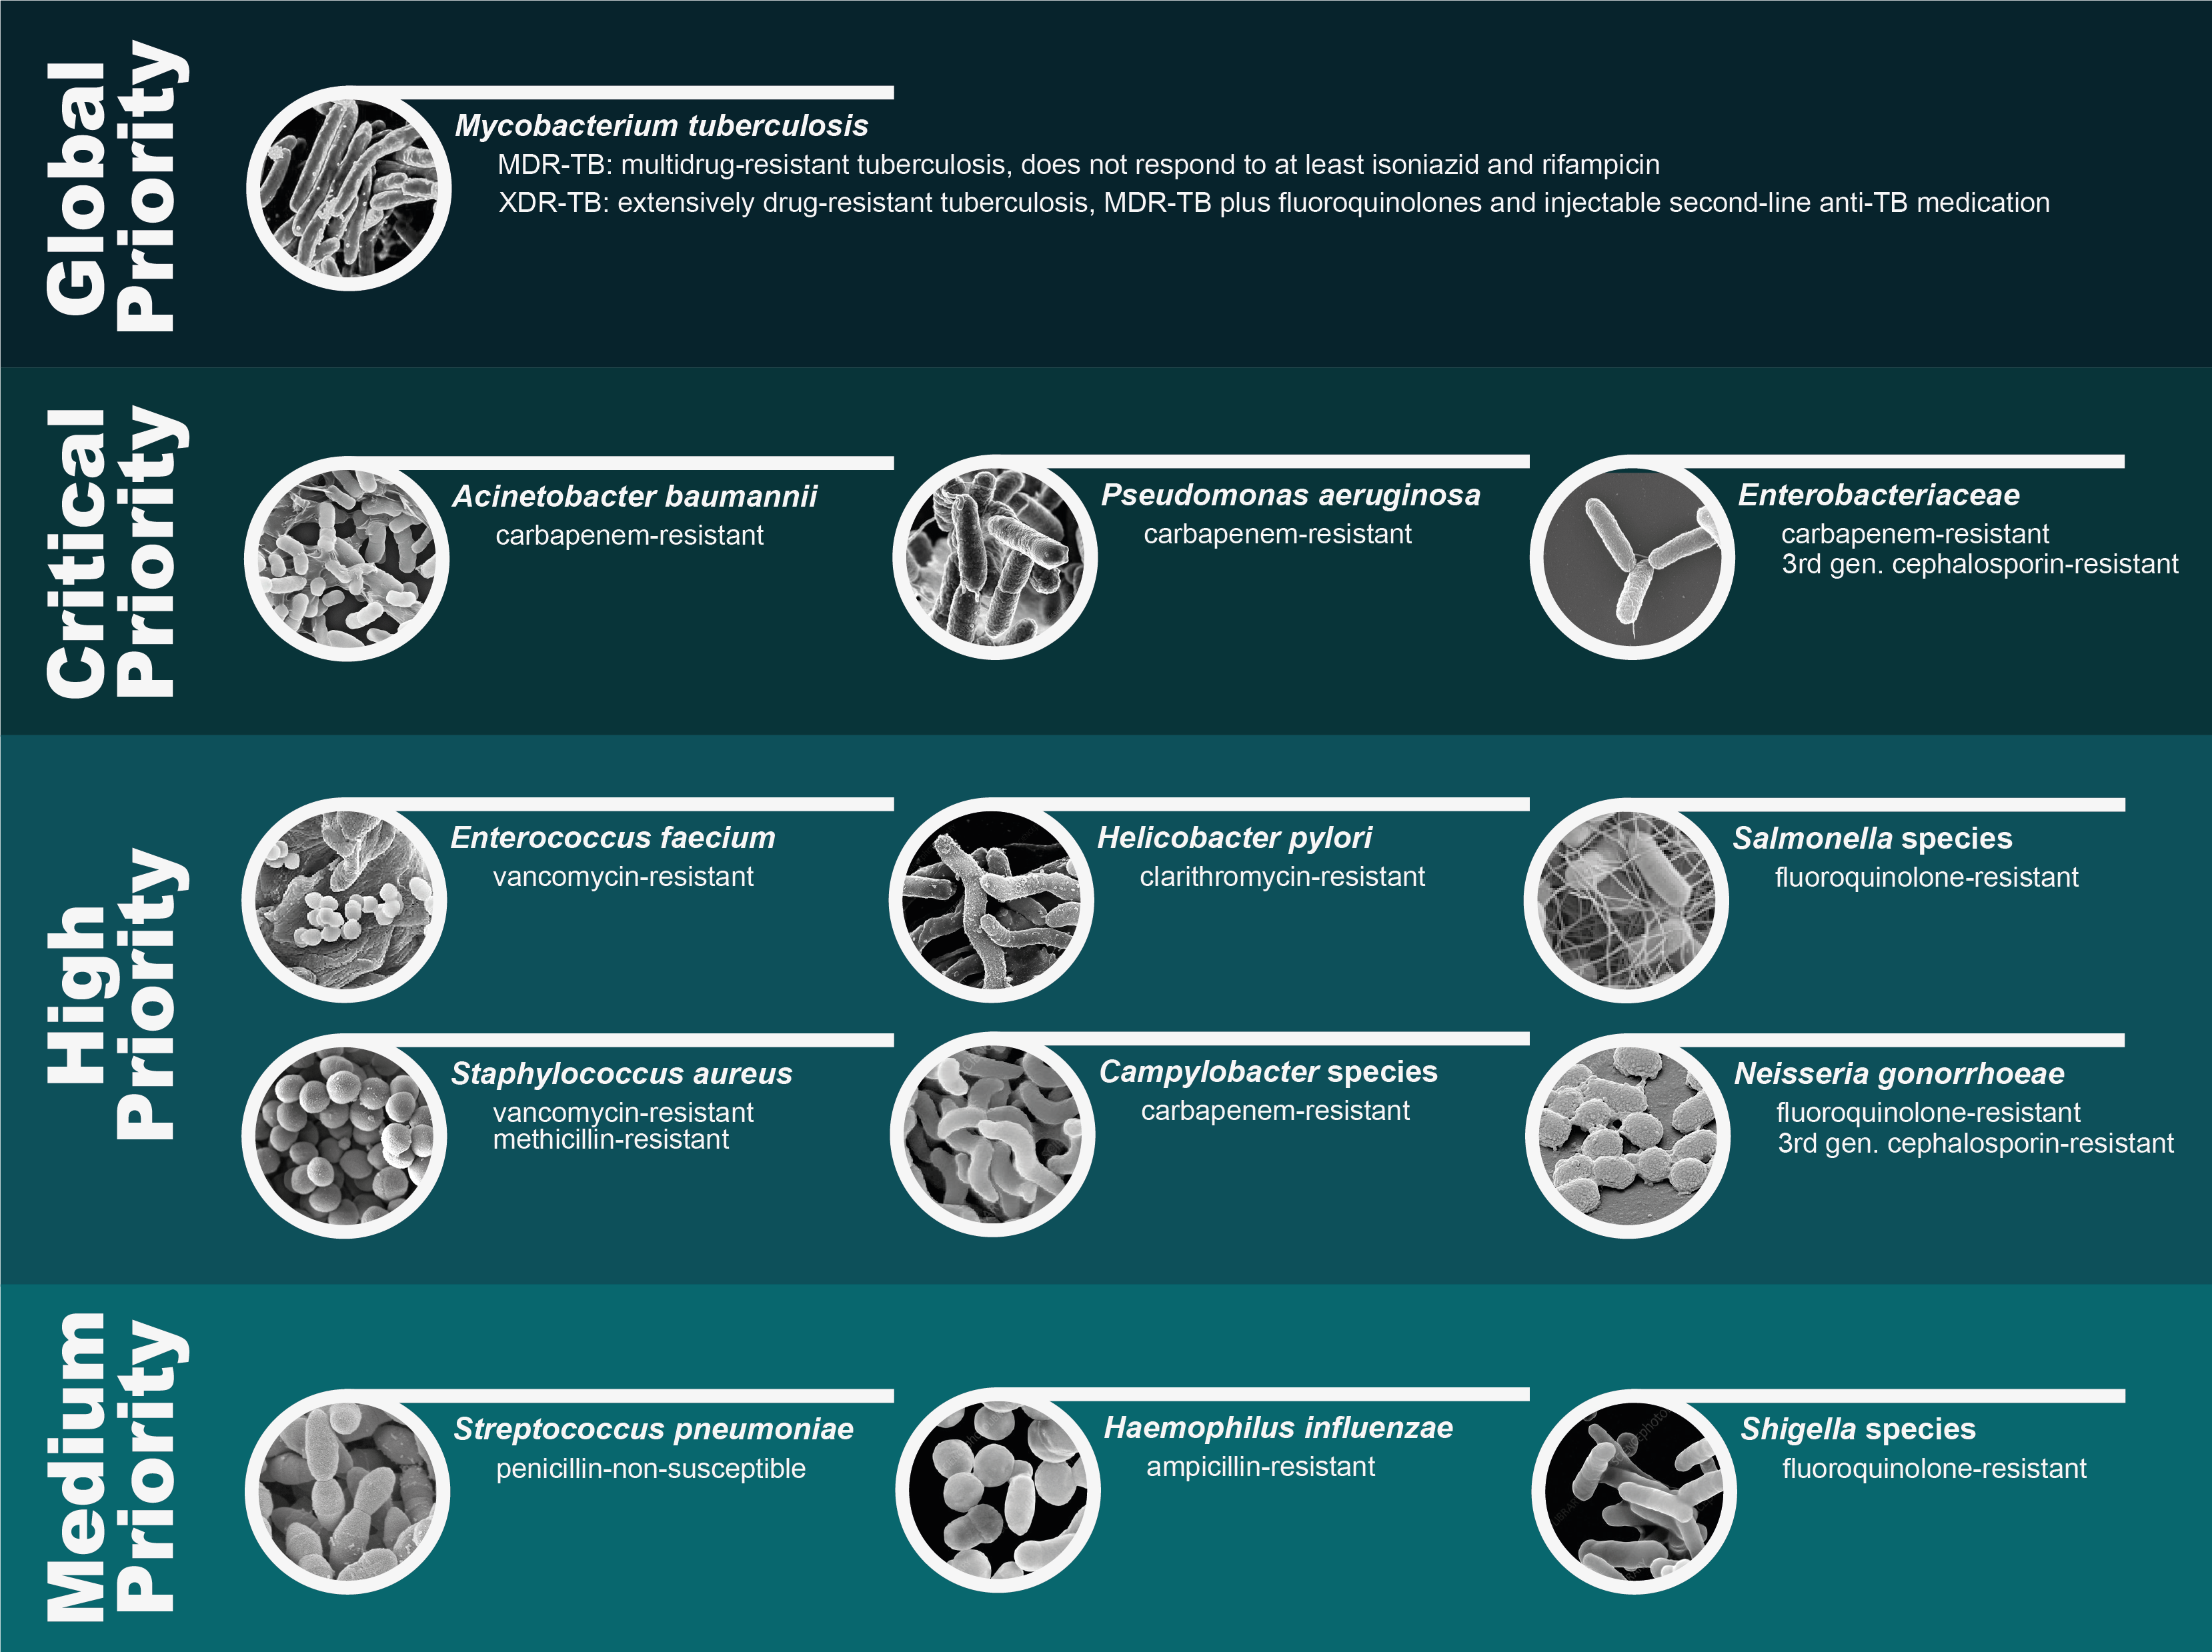
\includegraphics[width=\textwidth]{figures/introduction/Figure 1.pdf}
\caption{\textbf{World Health Organisation Global Priority Pathogens list.} This catalogue includes, besides \textit{Mycobacterium tuberculosis} considered the number one global priority, a list of twelve microorganisms grouped under three priority tiers according to their antimicrobial resistance: critical (\textit{Acinetobacter baumannii}, \textit{Pseudomonas aeruginosa} and \textit{Enterobacteriaceae}), high (\textit{Enterococcus faecium}, \textit{Helicobacter pylori}, \textit{Salmonella} species, \textit{Staphylococcus aureus}, \textit{Campylobacter} species and \textit{Neisseria gonorrhoeae}), and medium (\textit{Streptococcus pneumoniae}, \textit{Haemophilus influenzae} and \textit{Shigella} species). The major objective was to encourage the prioritisation of funding and incentives, align research and development priorities of public health relevance, and garner global coordination in the fight against antimicrobial resistant bacteria. Adapted from \cite{world_health_organization_prioritization_2017}.}
\label{fig:figure1}
\end{figure*}

Clinical microbiology is a discipline focused on rapidly characterising pathogen samples to direct the management of individual infected patients (diagnostic microbiology) and monitor the epidemiology of infectious disease (public health microbiology), including the detection of outbreaks and infection prevention. 
According to the \ac{WHO} Global Health Spending Report from 2000 to 2019, of the 51 countries that reported health spending by disease and condition, an average of 37\% of health spending went to infectious and parasitic diseases, corresponding to the largest share of health spending \citep{world_health_organization_global_2021}. 
About 21\% of total health spending went to three major infectious diseases - HIV / AIDS (9\%), tuberculosis (1\%) and malaria (11\%) - and 16\% went to other infectious and parasitic diseases. 
On average, 70\% of external health aid went to infectious and parasitic diseases in 51 low- and middle-income countries. 
Of the \$54.8 billion estimated disbursed for health in 2020, \$13.7 billion (25\%) was targeted toward the COVID-19 health response \citep{micah_tracking_2021}.

\subsection{Current standards for diagnostic in clinical microbiology} \label{ssec:_intro_current_standards}

The past few decades have seen a major revolution in the operation of microbial laboratories, driven by the development of molecular technologies and ways to make these accessible, namely amplification-based \ac{PCR}, matrix-assisted laser desorption/ionisation - time of flight (MALDI-TOF) and \ac{DNA}-microarray-based hybridisation technology. 
These are used in conjunction with traditional techniques such as microscopy, culture, and serology.
Application of these methods differs by suspected infection type: bacterial, viral, fungal or parasitic. 
For the purpose of this dissertation work, we will focus on bacterial (see Section \ref{sssec:_intro_bacterial}) and viral infections (see Section \ref{sssec:_intro_viral}).

\subsubsection{Bacterial infections} \label{sssec:_intro_bacterial}

For patients with bacterial infections, the crucial steps are (1) to grow an isolate from a specimen, (2) identify its species, and (3) determine its pathogenic potential and test its susceptibility to antimicrobial drugs  \citep{didelot_transforming_2012}. 
Together, this information facilitates the specific and rational treatment of patients. 
For public health purposes, knowledge also needs to be gained about (4) the relatedness of the pathogen to other strains of the same species to investigate transmission routes and allow recognition of outbreaks \citep{foxman_choosing_2005} (see Figure \ref{fig:figure2}). 

\begin{figure*}[h!]
\centering
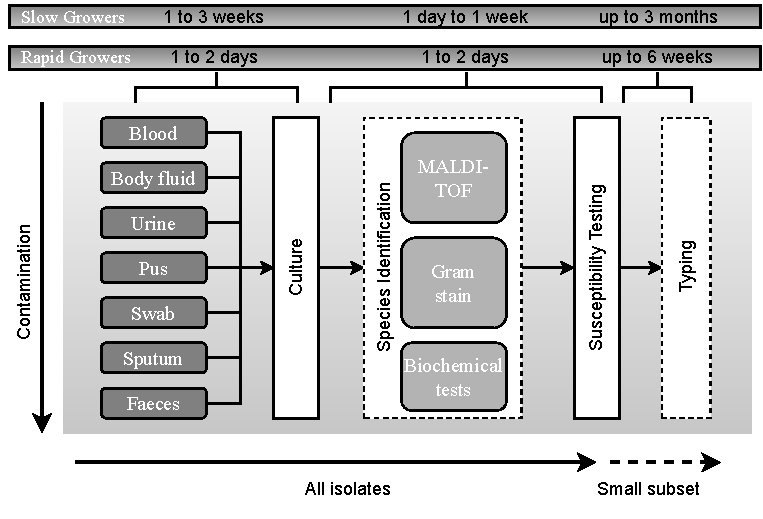
\includegraphics[width=\textwidth]{figures/introduction/Figure 2.pdf}
\caption{\textbf{Principles of current processing of bacterial pathogens.} Schematic representation of the current workflow for processing samples for bacterial pathogens is presented, with high complexity and a typical timescale of a few weeks to a few months. Samples that are likely to be normally sterile are often cultured on rich medium that will support the grown of any culturable organism. Samples contaminated with colonising flora present a challenge for growing the infecting pathogen. Many types of culture media (referred to as selective media) are used to favour the growth of the suspected pathogen.
Once an organism is growing, the likely pathogens are then processed through a complex pathway that has many contingencies to determine species and antimicrobial susceptibility. Broadly, there are two approaches. One approach uses MALDI-TOF for species identification prior to setting up susceptibility testing. The other uses Gram staining followed by biochemical testing to determine species; susceptibility testing is often set up simultaneously with doing biochemical tests. Lastly, depending on the species and perceived likelihood of an outbreak, a small subset of isolates may be chosen for further investigation using a wide range of typing tests. Adapted from \cite{didelot_transforming_2012}.}
\label{fig:figure2}
\end{figure*}

The current gold standard for bacterial pathogen identification in diagnostic microbiology laboratories involves the isolation of the pathogen through culture followed by biochemical testing, a multi-step process that can take days to weeks before obtaining results, depending on the fastidiousness of the organism and if it can be cultured \citep{muhamad_rizal_advantages_2020, giuliano_guide_2019, muhamad_rizal_advantages_2020}. 
Although culture allows the identification of a wide variety of organisms, some pathogens can escape routine investigation due to strict metabolic necessities for growth or the requirement for specific biochemical tests needed for their identification. 
Furthermore, results will be obscured if a mixed culture is obtained, particularly if the cultures are obtained from sites with a microbiota, such as the gut and the skin, increasing the risk of contamination by normal flora and leading to false results \citep{giuliano_guide_2019}. 
After successful growth in culture, Gram staining and MALDI-TOF mass spectrometry are often used for identification with good accuracy as long as the pathogen is presented in the the coexisting database \citep{patel_maldi-tof_2015}. 
An alternate rapid identification method is \ac{PCR} where nucleic acid fragments are detected through specific primers, being highly sensitive and specific, to the point where \ac{PCR} may detect bacteria that are not viable after a patient has been treated for an infection and it is limited to the primer used \citep{scerbo_beyond_2016}. 
Syndromic panels, an extension of \ac{PCR} by using multiple primers (multiplex \ac{PCR}) to simultaneously amplify nucleic acids from multiple targets in a single reaction, tried to address this issue by allowing for the identification of multiple bacteria and other important information such as the detection of antibiotic resistance or virulence genes \citep{giuliano_guide_2019}.

Following identification, antibiotic-susceptibility testing is essential to guide clinicians in selecting an appropriate treatment. 
Conventional methods of bacterial resistance detection, such as disc diffusion, antimicrobial gradient strip, and broth microdilution, are widely used, but results cannot be obtained before 48 hours after receiving a sample, which can lead to prolonged use or overuse of broad-spectrum antibiotics \citep{benkova_antimicrobial_2020}. 
Similarly to bacterial identification, MALDI-TOF and \ac{PCR} have been increasingly adopted as solutions with shorter turnaround times, although no phenotypic information is recovered, nor information on the minimum inhibitory concentration (MIC) for a given antibiotic.   

Choosing an appropriate bacterial typing technique for epidemiological studies depends on the available resources and the minimum intended resolution, ranging from \ac{DNA} fingerprinting to multilocus sequence typing, \ac{PFGE}, and sequence-based typing (see \secref{sec:_intro_genomics_approach}) \citep{allerberger_molecular_2012,foxman_choosing_2005}. 
\ac{DNA} macrorestriction analysis by \ac{PFGE}, which revolutionised precise separation of \ac{DNA} fragments, became the most widely implemented \ac{DNA} fingerprinting technique \citep{allerberger_molecular_2012}, becoming the golden standard for bacterial typing \citep{neoh_pulsed-field_2019}.

In the early 2000s, \ac{MLST} was proposed as a portable, universal, and definitive method for characterising bacteria \citep{maiden_multilocus_2006}. 
Instead of enzyme restriction of bacteria \ac{DNA}, separation of restricted \ac{DNA} bands using a \ac{PFGE} chamber, followed by clonal assignment of bacteria based on banding patterns, \ac{MLST} relies on the amplification through \ac{PCR} sequences of internal fragments of housekeeping genes (usually 5 to 7), approximately 450-500 \ac{bp} in size, followed by its sequence, usually my Sanger methods (see \secref{ssec:_intro_1st_gen_seq}). 
For each house-keeping gene, the different sequences present within a bacterial species are assigned as distinct alleles and, for each isolate, the alleles at each of the (usually) seven loci define the allelic profile or sequence type \citep{larsen_multilocus_2012}. 
As with \ac{PFGE}, different schemes, defining what housekeeping gene fragments are used, are available depending on the species. 
Unlike \ac{PFGE}, the provision of freely accessible, curated databases of \ac{MLST} nucleotide sequence data enables the direct comparison of bacterial isolates, providing the basis of a common language for bacterial typing \citep{maiden_multilocus_2006}. 
So far, \ac{MLST} schemes for more than 100 bacterial organisms have been published and made freely available\footnote{\url{https://pubmlst.org/organisms}}, \cite{jolley_open-access_2018}) 

Depending on the organism identified, further and/or particular typing schemes can be applied. 
For \textit{S. pneumoniae}, one of the pathogens listed in the \ac{WHO} \ac{GPP} list, the typing of the polysaccharide capsule, usually through Quellung reaction, is paramount for disease surveillance and evaluation of the pre- and post-pneumococcal vaccine, since the capsule, with over 90 serotypes reported, is the dominant surface structure of the organism and plays a critical role in virulence \citep{jauneikaite_current_2015, paton_streptococcus_2019}. 
For the \textit{Salmonella} species, also in the \ac{GPP} list, the serotype is usually determined by agglutination of the bacteria with specific antisera to identify variants of somatic (O) and flagella (H) antigens that, in various combinations, characterise more than 2600 reported serotypes \citep{diep_salmonella_2019}. 

\subsubsection{Viral infections} \label{sssec:_intro_viral}

Traditional approaches to laboratory diagnosis of viral infections have been (1) direct detection in patient material of virions, viral antigens, or viral nucleic acids, (2) isolation of the virus in cultured cells, followed by identification of the isolate, and (3) detection and measurement of antibodies in patient serum (serology) \citep{burrell_laboratory_2017}. 
Viral diagnostics is therefore generally organised into two primary categories, indirect and direct detection, depending on the method used \ref{fig:figure_viral}. 

\begin{figure*}[h!]
\centering
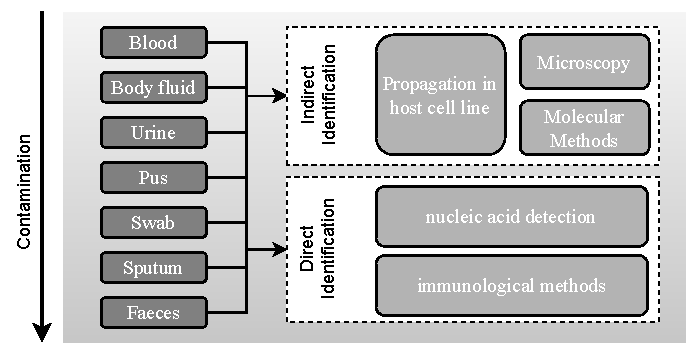
\includegraphics[width=\textwidth]{figures/introduction/viral.pdf}
\caption{\textbf{Principles of current processing of viral pathogens.} Schematic representation of the current workflow for processing samples for viral pathogens is presented. Samples that are likely to be normally sterile are often cultured and isolated in suitable host cell lines (indirect identification). This supports the identification through microscopy of molecular methods, but the virus can take weeks to propagate. Direct identification is much faster, relying on nucleic acid detection of immunologic assays for the identification of the pathogen, without the need of virus propagation.}
\label{fig:figure_viral}
\end{figure*}

Indirect detection methods involve the propagation of virus particles through their introduction to a suitable host cell line (virus isolation), since viruses rely on host organisms to replicate. 
This is a relatively slow diagnostic method, sometimes taking weeks for the virus to propagate, usually followed by microscopy for its identification, or more commonly, through molecular methods with an agent that detects a virus-associated protein, such as an antibody \citep{cassedy_virus_2021}. 

Direct detection methods negate the need for virus propagation, detecting the virus directly from the suspect source through nucleic acid and immunological methods. 
\ac{PCR} and \ac{RT-PCR} are widely applied methods for the detection of both \ac{DNA} and \ac{RNA} viruses, respectively, driven by increased awareness of the clinical value of and demand for prompt information about viral loads, viral sequence data and potential antiviral resistance information \citep{cassedy_virus_2021}. 
Syndromic testing (see \secref{sssec:_intro_bacterial}) is now fully integrated into standard testing practises of many clinical laboratories \citep{dien_bard_panels_2020}. 
The limitations of these assays include the absence of detection of off-target pathogens, a lack of full susceptibility information, cost, and false positive results. 
\ac{qPCR} remains the front line tool in aetiological diagnosis, measuring the production of the target amplicon throughout the reaction and providing quantitative results with high specificity and sensibility, albeit with a significant cost due to sophisticated apparatus despite high-throughput systems being widely established \citep{cassedy_virus_2021}.

Immunoassays employ singular-epitope specificity antibodies as the primary means to detect viruses within a sample and provide a much more cost-efficient alternative to nucleic acid detection \citep{cassedy_virus_2021}. 
A major application is seroprevalence assays, an essential technique to identify patients who have been exposed to a virus (historical exposure), detect asymptomatic infection, or evaluate the efficacy of vaccines \citep{chan_determining_2021, bobrovitz_global_2021}. 
\ac{LFIA} are widely used to detect virus-associated proteins directly from the source through antibodies labelled that binding to their cognate antigens, usually read by means of a colour change at a test line. 
In addition to being very cost-effective, \ac{LFIA} have a turnaround time of minutes and the colour change can be observed with the naked eye, therefore facilitating rapid diagnosis, but their results are limited to semiquantitative and typically do not achieve sensitivity comparable to nucleic acid detection \citep{estrela_lateral_2016, cassedy_virus_2021, di_nardo_ten_2021}.

\subsection{Surveillance and infection prevention in public health} \label{ssec:_intro_survaillance}

Infectious disease surveillance is critical for improving population health, generating information that drives action not only in the management of infected patients but also in the prevention of new ones by identifying emerging health conditions that may have a significant impact by (1) describing the current burden and epidemiology of the disease, (2) to monitoring trends, and (3) identifying outbreaks and new pathogens \citep{groseclose_public_2017, murray_infectious_2017}. 
\ac{PHSS} consist of the ongoing systematic collection, analysis and interpretation of data, and its integration with the timely dissemination of results to those who can carry out effective prevention and control activities \citep{teutsch_considerations_2010}. 

Traditional \ac{PHSS} can have different approaches based on the epidemiology and clinical presentation of the disease and the goals of surveillance. 
In passive surveillance systems, medical professionals in the community and health facilities report cases to the public health agency, which conducts data management and analysis once the data is received and communicates with the responsible entities. 
Globally, the \ac{WHO} as described in the International Health Regulations what is notifiable by all countries, such as severe acute respiratory syndrome (SARS) and viral hemorrhagic fevers (Ebola, Lassa, Marburg), as well as guiding which public health measures should be implemented \citep{world_health_organization_international_2005}. 
Active surveillance aims to detect every case, not relying on a reporting structure, and can have many approaches from sentinel sites or network of sites that capture cases of a given condition, such as respiratory tract infections, within a catchment population \citep{murray_infectious_2017, melo-cristino_estudo_2006}. 
The application of environmental surveillance methods, performed prospectively to detect pathogens prior to the recording of clinical cases or to monitor their abundance in the environment to assess the potential risk of disease, has been proven as a viable alternative, particularly in wastewater \citep{andrews_environmental_2020, mcweeney_demonstration_1894, baker_combined_2011, larsen_tracking_2020}.  

The emergence and reemergence of infectious diseases are closely linked to the biology and ecology of infectious agents, their hosts, and their vectors \citep{destoumieux-garzon_one_2018}.
"One Health" is a collaborative and multi-disciplinary approach to designing and implementing programmes, policies, legislation and research in which multiple sectors communicate and work together to achieve better public health outcomes \citep{mackenzie_one_2019}. 
It recognises that people's health is closely related to the health of animals and the shared environment, focussing on zoonotic and vector-borne diseases, antimicrobial resistance, food safety, food security, and environmental contamination \citep{rugarabamu_one-health_2021}.
This is crucial to (1) understanding the emergence and re-emergence of infectious and noncommunicable chronic diseases and (2) in creating innovative control strategies.
A better understanding of the causes and consequences of certain human activities, lifestyles, and behaviours in ecosystems is crucial for a rigorous interpretation of disease dynamics and to drive public policies, but it requires breaking down the interdisciplinary barriers that still separate human and veterinary medicine from ecological, evolutionary, and environmental sciences \citep{destoumieux-garzon_one_2018}. 

\section{A genomic approach to clinical microbiology} \label{sec:_intro_genomics_approach}

Since the publication of the first complete microbial genome, a quarter of a century ago, of the bacterium \textit{Haemophilus influenzae} \citep{hood_dna_1996}, genomics has transformed the field of microbiology, and in particular its clinical application (see Figure \ref{fig:figure3}). 

\begin{figure*}[h!]
\centering
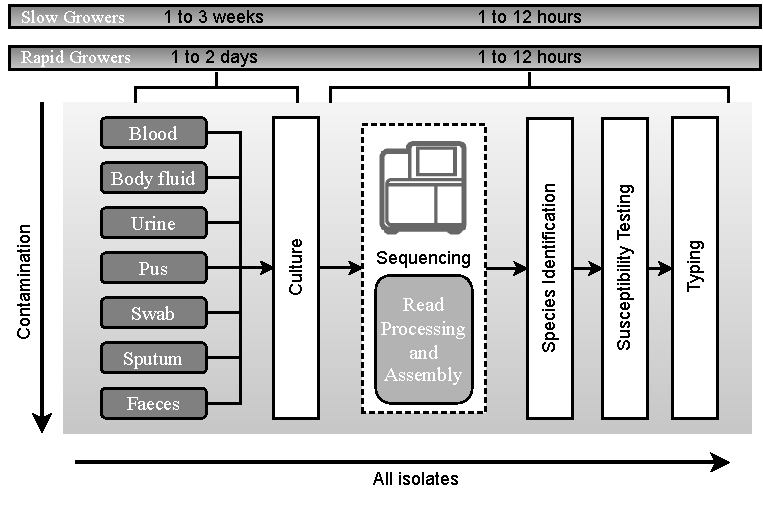
\includegraphics[width=\textwidth]{figures/introduction/Figure 3.pdf}
\caption{\textbf{Principles of current processing of bacterial pathogens based on whole genome sequencing.} Schematic representation of the workflow for processing samples for bacterial pathogens after the adoption of whole genome sequencing, with an expected timescale that could fit within a single day. The culture steps would be the same as currently used in a routine microbiology laboratory (see Figure \ref{fig:figure2}). Once a likely pathogen is ready for sequencing, \ac{DNA} is extracted, taking as little as 2 hours to prepare the \ac{DNA} for sequencing.
After sequencing, the main processes for yielding information is computational. Automated sequence assembly algorithms are necessary for processing the raw sequence data, from which species, relationship to other isolates of the same species, antimicrobial resistance profile and virulence gene content can be assessed. All the results can also be used for outbreak detection and infectious diseases surveillance. Adapted from \cite{didelot_transforming_2012}}
\label{fig:figure3}
\end{figure*}

The paper describing the \ac{DNA}-sequencing method with chain-terminating inhibitors used in the sequencing of the first microbial genome \citep{sanger_dna_1977}, which earned the late Frederick Sanger his share of the 1980 Nobel Prize in Chemistry alongside Walter Gilbert, was, in 2014, the top fourth in the number of citations with over 60000, highlighting its impact in the field of biological sciences, and by extension medicine \citep{van_noorden_top_2014}. 
Currently, this number has increased to over 84000 according to \ac{PMC}\footnote{\url{https://pubmed.ncbi.nlm.nih.gov/}}\footnote{\url{ https://www.ncbi.nlm.nih.gov/pmc/articles/PMC431765/}}. 
Since its emergence, reductions in cost, technical advances in sequencing technologies, and new computational developments have made genomic sequencing one of the most influential tools in biomedical research, yielding unprecedented insights into microbial evolution and diversity, and the complexity of the genetic variation in both commensal and pathogenic microbes. 
The emerging application of genomic technologies in the clinic to combat infectious diseases is transforming clinical diagnostics and the detection and surveillance of outbreaks. 

\subsection{Twenty five years of microbial genome sequencing} \label{ssec:_intro_sequencing}

Since the discovery of the structure of \ac{DNA} \citep{watson_molecular_1953}, great strides have been made in understanding the complexity and diversity of genomes in health and disease. 
The development and commercialisation of high-throughput, massively parallel sequencing has democratised sequencing by offering individual laboratories, either in research or in health, access to the technology. 
Over the last quarter of a century, three main revolutions can be considered in genomic sequencing: the first, the second and the third generations of sequencing (see Figure ~\ref{fig:figure5}).

\begin{figure*}[h!]
\centering
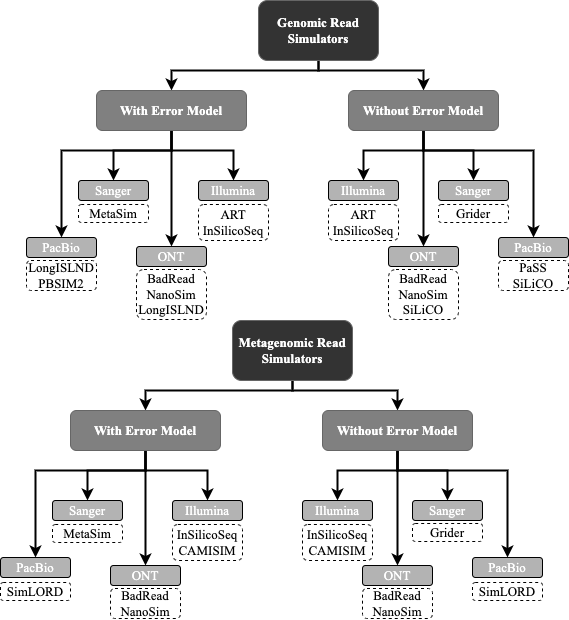
\includegraphics[width=\textwidth]{figures/introduction/Figure 5.png}
\caption{\textbf{The three revolutions in sequencing technology that have transformed the landscape of bacterial genome sequencing.} The first-generation, also known as Sanger sequencers, is represented by the ABI Capillary Sequencer (Applied Biosystems). During the sequencing reaction, at each nucleotide incorporation event, a fluorescently labelled \ac{ddNTP} is incorporated, terminating the elongation of the \ac{DNA} molecule. The resulting electropherogram for sequencing reaction is below, and is read from left to right. The second-generation, also known as high-throughput sequencers, is represented by MiSeq, a 4-channel sequencer, and NextSeq, a 2-channel sequencer (Illumina), both sequencing by synthesis instruments. For both instruments, the loaded flowcell is sequenced in massive parallel reactions, with each nucleotide incorporation emitting a light signal that is captured and latter basecalled into a fastq file, with indication of the confidence of the call, presented below. In a 4-channel instrument each nucleotide has its own marker (A: yellow, T: green, C: red, G: blue) but in a 2-channel instrument only 2 markers exist (A: green plus red, T: green, C: red, G: no marker). These instruments allow the sequencing of both ends of the \ac{DNA} fragment. Lastly, the third-generation, also known as long-read sequencers, is represented by the Pacific Bioscience BS sequencer and Oxford Nanopore MinION sequencer. In the first, immobilised polymerases in a \ac{SMRT} Cell incorporating nucleotides with identifying fluorescent labels. In the latter, a nanopore embedded in a solid-state membrane causes a change in an ionic current across the membrane each time a nucleotide is pushed through the pore. This difference in potential is then used for basecalling. Adapted from \cite{hagemann_overview_2015, loman_twenty_2015,goodwin_coming_2016, wang_nanopore_2021, metzker_sequencing_2010, xu_recent_2020}}
\label{fig:figure5}
\end{figure*}

\subsubsection{The first-generation of DNA sequencing} \label{ssec:_intro_1st_gen_seq}

In the late 1980s, automated Sanger sequencing machines could sequence approximately 1,000 bases per day, having been applied in the 1990s to large bacterial genomes and the first unicellular and multicellular eukaryotic genomes \citep{koch_sequencing_2021}. 
The first genomes of pathogenic \textit{Mycobacterium tuberculosis} \citep{cole_deciphering_1998}, \textit{Yersinia pestis} \citep{parkhill_genome_2001}, \textit{Escherichia coli} K-12 \citep{blattner_complete_1997} were sequenced using this technology, requiring years of effort and significant budgets, but providing insights into the genomic complexity of these organisms. 
Some of the complete genome sequences produced during this era are still used today as high-quality references. 

Simplistically, in first-generation \ac{DNA} sequencing, also known as Sanger sequencing, a \ac{DNA} polymerase is used to synthesise numerous copies of the sequence of interest using \ac{ddNTP}) in the reaction. 
At each nucleotide incorporation event, there is a chance that a \ac{ddNTP} will be added and the growing \ac{DNA} chain will terminate, resulting in a collection of \ac{DNA} molecules of varying lengths \citep{sanger_dna_1977, hagemann_overview_2015}. 
Modern Sanger sequencing uses fluorescently labelled \ac{ddNTP} that allow the amplification step to be performed in a single reaction, resulting in a mixture of single-stranded \ac{DNA} fragments of various lengths, each tagged at one end with a fluorophore indicating the identity of the 3' nucleotide that, after separation through capillary electrophoresis, the resulting electropherogram with four-colour fluorescence intensity can be interpreted by a base-calling software and producing 600–1000 bases of accurate sequence per reaction\citep{hagemann_overview_2015}. 

The first generation sequencing technology remains very useful for applications where high-throughput is not required due to its cost-effectiveness, relatively low sample load and accuracy of sequencing, even in repetitive genomic regions, although input \ac{DNA} must consist of a relatively pure population of sequences \citep{slatko_overview_2018}. 
One of the most common uses is thus individual sequencing reactions using a specific \ac{DNA} primer on a specific template, such as \ac{MLST} of bacterial genomes. 

\subsubsection{The second-generation of DNA sequencing} \label{ssec:_intro_2nd_gen_seq}

The release of the first truly high-throughput sequencing platform in the mid-2000s heralded a 50,000-fold drop in the cost of \ac{DNA} sequencing in comparison with the first-generation technologies and led to the denomination of the second generation as next-generation sequencing (NGS) \citep{goodwin_coming_2016}. 
This trend has continued over the next two decades of continued development and improvement, allied to the emergence of benchtop sequencing platforms with a high-throughput sequencing data and turnaround times of days, making it a standard in any microbiology and public health laboratories \citep{loman_twenty_2015}. 
Second-generation sequencing methods can be grouped into two major categories: (1) sequencing by hybridisation and (2) sequencing by synthesis. 

\paragraph{Sequencing by hybridisation} \label{sssec:_intro_2nd_gen_seq_hybrid} \mbox{}\\

Sequencing by hybridisation, also known as sequencing by ligation, originally developed in the 1980s, relies on the binding of one strand of \ac{DNA} to its complementary strand (hybridisation). 
By repeated hybridisation and washing cycles, it was possible to build larger contiguous sequence information, based on overlapping information from the probe hybridisation spot, being sensitive to even single-base mismatches when the hybrid region is short or if specialised mismatch detection proteins are present \citep{slatko_overview_2018, detter_nucleic_2014}. 
Although widely implemented via \ac{DNA} chips or microarrays, has largely been displaced by other methods, including sequencing by synthesis \citep{goodwin_coming_2016}. 

\paragraph{Sequencing by synthesis} \label{sssec:_intro_2nd_gen_seq_synth} \mbox{}\\

Sequencing by synthesis methods is a further development of Sanger sequencing, without the \ac{ddNTP} terminators, in combination with repeated cycles, run in parallel, of synthesis, imaging, and methods to incorporate additional nucleotides in the growing chain. 
All second-generation sequencing by synthesis approaches relies on a ‘library’ preparation using native or amplified \ac{DNA} usually obtained by (1) \ac{DNA} extraction, (2) \ac{DNA} fragmentation and fragment size selection, and (3) ligation of adapters and optional barcodes to the ends of each fragment. 
This is generally followed by a step of \ac{DNA} amplification. The resulting library is (4) loaded into a flow cell and (5) sequenced in massive parallel sequencing reactions \citep{giani_long_2020}.
Besides having much shorter read lengths than first-generation methods, with reads ranging from 45 to 300 bases,. These have an intrinsically higher error rate, the massively parallel sequencing of millions to billions of short \ac{DNA} sequence reads allows the obtainment of millions of accurate sequences based on the identification of consensus (agreement) sequences \citep{slatko_overview_2018, goodwin_coming_2016, hagemann_overview_2015}. 

Many of the approaches currently available for sequencing by synthesis methods have been described as cyclic array sequencing platforms, as they involve dispersal of target sequences across the surface of a two-dimensional array, followed by sequencing of those targets \citep{hagemann_overview_2015}. 
They can also be classified as single nucleotide addition or cyclic reversible termination or as single nucleotide addition \citep{goodwin_coming_2016}. 

The first relies on a single signal to mark the incorporation of a \ac{dNTP} into an elongating strand, avoiding the use of terminators. 
As a consequence, each of the four nucleotides must be added iteratively to a sequencing reaction to ensure that only one \ac{dNTP} is responsible for the signal. 
The Roche 454 Life Sciences pyrosequencing device \footnote{\url{https://web.archive.org/web/20161226040638/http://454.com/}, snapshot from 26 December 2016}, was the first and most popular instrument implementing this technology, but discontinued since 2013 with support to the platform ceasing in 2016. 
This system distributes template-bound beads into a PicoTiterPlate along with beads containing an enzyme cocktail. 
As a \ac{dNTP} is incorporated into a strand, an enzymatic cascade occurs, resulting in a bio-luminescence signal which is captured by a camera, which can be attributed to the incorporation of one or more identical \ac{dNTP}s at a particular bead \citep{goodwin_coming_2016}. 
The ThermoFisher Ion Torrent system \footnote{\url{https://www.thermofisher.com/pt/en/home/brands/ion-torrent.html}}, released in 2010 and still available today, replaces the optical sensor, using instead  H+ ions that are released as each \ac{dNTP} is incorporated in the enzymatic cascade, and the consequential change in pH, to detect a signal \citep{goodwin_coming_2016}. 
Alongside the 454 pyrosequencing system, this system has difficulty in enumerating long repeats, additionally, the throughput of the method depends on the number of wells per chip, ranging from 10 megabases to 1000 megabases of 100 base reads in length, but with a very short run time (three hours) \citep{hagemann_overview_2015, loman_performance_2012}.

The latter is defined by their use of terminator molecules that are similar to those used in the first-generation of sequencing, preventing elongation of the DNA molecule, but unlike the first methods, it is reversible. 
To begin the process, a \ac{DNA} template is primed by a sequence that is complementary to an adapter region, which will initiate polymerase binding to this double-stranded \ac{DNA} region. 
During each cycle, a mixture of all four individually labelled and 3'-blocked \ac{dNTP}s are added. 
After incorporation of a single \ac{dNTP} into each elongating complementary strand, the unbound \ac{dNTP}s are removed and the surface is imaged to identify which \ac{dNTP} was incorporated at each cluster by optical capture. 
The fluorophore and blocking group can then be removed and a new cycle can begin \citep{goodwin_coming_2016}. 
The Illumina systems, which use this technology, accounts for the largest market share for sequencing instruments compared to other platforms\footnote{\url{https://www.forbes.com/companies/illumina/?sh=774358a91aa6}}, allowing paired-end sequencing and having the highest throughput (from 25 million reads for a MiSeq instrument to  1.2 billion reads for a NextSeq instrument\footnote{\url{https://www.illumina.com/systems/sequencing-platforms.html}}), with read lengths ranging from 45 to 300 bases in length with high accuracy, albeit with long running times (4 to 55 hours), rendering this technology a good choice for many sequencing applications where large read length is not required \citep{loman_performance_2012, gupta_chapter_2014, hagemann_overview_2015}.

\subsubsection{The third-generation of DNA sequencing} \label{ssec:_intro_3rd_gen_seq}

Despite their wide adoption, second-generation methods require in the library preparation an enrichment or amplification step. 
These steps are time-consuming, introduce biases related to preferential capture or amplification of certain regions, and produce reads with relatively small size, making transversing repetitive genomic regions impossible if they are larger than the read length \citep{hagemann_overview_2015}. 
Third-generation sequencing technologies, also known as long-read sequencing or single-molecule sequencing, are characterised by the generation of ultra-long-reads, albeit at a much lower throughput than the second-generation \citep{hoang_long-reads-based_2022}. 
They also have the potential to go beyond four-base sequencing to reveal genome-wide patterns of methylation and other chemical modifications that control the biology or the virulence of pathogens \citep{korlach_going_2012}. 
Currently, commercial long-read sequencing is supported by two companies: \ac{PacBio}\footnote{\url{https://www.pacb.com/}} and \ac{ONT}\footnote{\url{https://nanoporetech.com/}}. 

The basis of \ac{PacBio} sequencers is known as \ac{SMRT}, which takes place in single-use \ac{SMRT} Cells. 
These contain multiple immobilised polymerases, which, after binding to an adaptor sequence, begin replication incorporating nucleotides with identifying fluorescent labels. 
The sequence of fluorescence pulses is recorded into a movie which is then converted into a nucleotide sequence. 
After the polymerase completes replication of one \ac{DNA} strand, it continues to sequence the opposite adapter and second strand. 
As a result, multiple passes of the same template can be generated depending on the lifetime of the polymerase \citep{hoang_long-reads-based_2022, loman_twenty_2015}. 
This technology has accuracy comparable with the Illumina systems but requires a higher initial investment cost, are much larger machines in comparison with the benchtop counterparts, and have much lower throughput and longer library preparation protocols \citep{hoang_long-reads-based_2022, wenger_accurate_2019}. 

\ac{ONT} makes use of nanopores in small, portable single-molecule sequencing devices, capable of generating ultra-long sequences in real-time at a relatively low cost. 
Biological nanopores are embedded in solid-state membranes within disposable flow cells which, when a \ac{DNA} strand passes through the pore driven by a motor protein, each nucleotide causes a change in an ionic current across the membrane, which is later base called \citep{hoang_long-reads-based_2022, loman_twenty_2015}. 
This process is free from fluorescence labels and amplification requirements, and after one strand is processed, the pore is available to sequence the next available strand. 
Sequence quality and length depend on the loaded library but are usually much lower than the alternative counterparts, and its throughput is dependent on the number and lifespan of the nanopore within the flowcell, but still much lower than the alternatives. 
Despite this, its portability, fast advances, and continued improvement of the flowcells make this a fast adopted technology for long-read sequencing.  

\subsection{DNA sequencing in clinical diagnosis and surveillance} \label{ssec:_intro_sequencing_diagnosis}

\ac{WGS} is becoming one of the most widely used applications of microbial genome sequencing. 
The major advantage of \ac{WGS} is to yield all the available \ac{DNA} information content on isolates in a single rapid step following culture (sequencing without culture will be discussed in the \secref{ssec:_intro_metagenomics}). 
In principle, after obtaining a pure culture, either bacterial (see \secref{sssec:_intro_bacterial}) or viral (see \secref{sssec:_intro_viral}), the data from sequencing contain all the information currently used for diagnostic and typing needs, and much more, thus opening the prospect for large-scale research into pathogen genotype-phenotype associations from routinely collected data \citep{didelot_transforming_2012}.
The cost of producing massive amounts of information requires a new framework with expert handling and processing of computer-driven genomic information, as well as capable computational infrastructures (see Section \ref{sec:_intro_bioinformatics}), but through this technology, researchers and clinicians can obtain the most comprehensive view of genomic information and associated biological implications, transforming clinical diagnostics and the detection and surveillance of outbreaks. \citep{cirulli_uncovering_2010, nature_reviews_genetics_genomic_2019, goodwin_coming_2016}.

Targeted sequencing is also proving invaluable to clinical microbial and research, not only by allowing more individual samples to be sequenced within a single run, significantly reducing costs and the amount of data generated, but also, due to the smaller target size, obtaining results with very high confidence due to the high coverage obtained \citep{goodwin_coming_2016}.
This has been particularly useful in viral genomics where sections, such as the capsid, or the complete viral genome can be selectively targeted directly from the suspected sample, offering a more time-effective method to achieve the same output as traditional nucleic acid amplification methods \citep{cassedy_virus_2021}. 

\subsubsection{Sequencing in the routine laboratory workflow} \label{sssec:_intro_sequencing_routine_lab}

\ac{WGS} has been used in the routine laboratory workflow when typing of pathogens by a method having the highest possible discriminatory power is required either through \ac{SNP} or \ac{cg/wg MLST} analysis, for example during hospital outbreaks \citep{tagini_bacterial_2017}. 

The implementation of \ac{WGS} in routine diagnostics requires several adaptations in the laboratory workflow, from the ‘wet’ laboratory part (extraction, library preparation, sequencing), to the ‘dry’ bioinformatics part where genomic data is analysed and its results interpreted by specialised personnel \citep{rossen_practical_2018}. 

Currently, sequencing technologies are used in a case-by-case approach, with its adoption being much more present in a research setting than in a diagnostic one. 
Sequencing is mostly used after a diagnostic through the identification of the causative agent has already been performed. 
Although substantial advances have been made in reducing response time, most of the current systems do not yet generate enough data fast enough for a truly rapid response for it to be used in the clinical setting \citep{goodwin_coming_2016}. 
High-throughput \ac{DNA} sequencing has found additional new applications in drug discovery and in functional genomics with, for example, SNP-based analysis to identify new drug targets \citep{loman_twenty_2015}.

Although the second-generation \ac{DNA} sequencing methods have shed light on fundamental aspects of microbial ecology and function, they suffer from issues associated with short read length (see \ref{ssec:_intro_2nd_gen_seq}) and cannot reliably reconstruct long repeats because of uncertainties in mapping read, even when paired-end sequencing is used. 
Third-generation sequencing methods (see \ref{ssec:_intro_3rd_gen_seq} The third-generation of \ac{DNA} sequencing) have become increasingly used in microbiology, although their accuracy and low throughput make it difficult to implement in a clinical diagnostic setting. 

\subsubsection{Sequencing and genomic surveillance} \label{sssec:_intro_sequencing_genomic_survaillance}

Most notably, \ac{WGS} has become a common tool in infection surveillance and prevention, allowing identification and tracking of pathogens, establishing transmission routes and outbreak control \citep{lo_genomics_2020}. 
In bacterial infections, initiatives such as Pathogenwatch\footnote{\url{https://pathogen.watch/}} offers a web-based platform for \ac{AMR} analysis and phylogeny generation of \textit{Campylobacter}, \textit{Klebsiella}, \textit{Neisseria gonorrhoeae}, \textit{Staphylococcus aureus}, and \textit{Salmonella Typhi} \citep{afolayan_overcoming_2021}. 
The Center for Genomic Epidemiology website\footnote{\url{https://www.genomicepidemiology.org/}} offers services for phylogenetic tree building and \ac{AMR} prediction. 
Chewie Nomenclature Server\footnote{\url{https://chewbbaca.online/}} allows users to share genome-based gene-by-gene typing schemas and to maintain a common nomenclature, simplifying the comparison of results \citep{mamede_chewie_2021}. 
Enterobase\footnote{\url{https://enterobase.warwick.ac.uk/}} allows for the analysis and visualisation of genomic variation within enteric bacteria \citep{zhou_enterobase_2020}. 
Microreact\footnote{\url{https://microreact.org/}}, from the same developers as Pathogenwatch, combines clustering, geographical and temporal data into an interactive visualisation with trees, maps, timelines and tables for a multitude of microorganisms, both bacterial and viral \citep{argimon_microreact_nodate}. 
Particularly for viruses, GISAID\footnote{\url{https://www.gisaid.org/}}  promotes the rapid sharing of data from all influenza viruses and the coronavirus causing COVID-19, including the genetic sequences and related clinical and epidemiological data \citep{shu_gisaid_2017}. 
ViPR\footnote{\url{https://www.viprbrc.org/}} provides access to sequence records, gene and protein annotations, immune epitopes, 3D structures, host factor data, and other data types for over 14 viral families, including \textit{Coronaviridae}, from which \ac{SARS-CoV-2} belongs to, and \textit{Faviviridae}, the family of Dengue and Zika virus \citep{pickett_virus_2012}. 
INSaFLU\footnote{\url{https://insaflu.insa.pt/}} supplies public health laboratories and influenza researchers with a web-based suite for effective and timely influenza and \ac{SARS-CoV-2} laboratory surveillance, identifying the type and subtype/lineage, detection of putative mixed infections and intra-host minor variants \citep{borges_insaflu_2018}. Nextrain\footnote{\url{https://nextstrain.org/}} provide a continually-updated view of publicly available data alongside powerful analytic and visualisation tools to aid epidemiological understanding and improve outbreak response for 10 pathogens: Influenza, SARS-CoV-2, West Nile virus, Mumps, Zika, West African Ebola, Dengue, Measles, Enterovirus D68 and Tuberculosis \citep{hadfield_nextstrain_2018}.

In outbreak detection and surveillance, genetic sequencing techniques combined with epidemiological data have undoubtedly provided immeasurable insights regarding evolutionary relationships and transmission pathways in various environments \citep{beckett_pandemic_2021, lancet_genomic_2021}. 
In a pandemic setting, this approach, although not novel, has been revolutionary, particularly in the COVID-19 setting. 

In the 2009 swine-origin Influenza A H1N1 pandemic, the first complete genome was publicly available on the 25 of April of 2009 (GenBank accession number FJ966079), about a month after records of increased flu activity in Mexico and 10 days after the first confirmed cases in California, United States of America \citep{smith_origins_2009, novel_swine-origin_influenza_a_h1n1_virus_investigation_team_emergence_2009}. 
By the time the pandemic was declared, on 11 of June of 2009, \cite{smith_origins_2009} reported the origins and evolutionary genomics of the pandemic influenza A variant with a collection of 813 complete influenza genome sets, 17 of which belonging to the newly swine influenza viruses (GenBank accessions numbers GQ229259–GQ229378). 
The \ac{MERS} pandemic, declared as such in 2015 \citep{piret_pandemics_2021}, had its first publicly available sequence on 5 of July 2015 (GenBank accession number KT006149)\citep{lu_complete_2015}, with a sequence from a camel, thought to be an intermediate host for the virus, available as early as 7 of March 2016 (GenBank accession number KU740200) \citep{kandeil_complete_2016, al-shomrani_genomic_2020}. 

The \ac{SARS-CoV-2} has brought a new meaning to genomic surveillance, with the first sequence from a COVID-19 patient being made publicly available as early as 12 January 2020 from a case of respiratory disease from the Wuhan outbreak (GenBank accession number MN908947) \citep{wu_new_2020}. 
At the date of the pandemic declaration by WHO, at 11 March 2020, over 400 complete \ac{SARS-CoV-2} sequences were deposited on GISAID\footnote{\url{http://web.archive.org/web/20200311053731/https://www.gisaid.org/}}, hitting over one million sequences in April 2021 \citep{maxmen_one_2021}. 
Currently, over 8 million complete viral sequences are available at GISAID\footnote{\url{https://www.gisaid.org/}}, being one of the most highly sequenced genomes of any organism on the planet. 
This richness in genomic information has been basal to identifying new variants of risk and new variants of concern with a myriad of different origins, identifying routes of transmission across borders, including the identification of "super-spreaders" events, and informing infection control measures \citep{lancet_genomic_2021, beckett_pandemic_2021, borges_sars-cov-2_2022}.  

\subsection{From genomics to metagenomics} \label{ssec:_intro_metagenomics}

Despite the increasing adoption of \ac{DNA} sequencing methods in clinical microbiology, the sequencing of genetic material from a pure culture requires \textit{a priori} knowledge of what to expect from a particular clinical sample or patient \citep{schuele_future_2021}. 
In most cases, this knowledge is enough to request the most appropriate test, such as syndromic panels or specific culture media, but this is not always the case. 
In recent years, there has been a growing interest in using metagenomics to deliver culture-independent approaches to microbial ecology, surveillance and diagnosis (see Figure \ref{fig:figure4})\citep{loman_twenty_2015, loman_high-throughput_2012}.
Metagenomic \ac{DNA} sequence allows detailed characterisation of pathogens in all kinds of samples originating from humans, animals, food and the environment, ligating the diagnostics to surveillance in a true "one health" fashion \citep{rossen__2018}. 
Unlike \ac{PCR} or microarrays, it usually does not require primer or probe design, it can be easily multiplexed, and the specificity and selectivity of the sequencing can be adjusted computationally after acquiring the data \citep{dunne_next-generation_2012} (see \ref{sec:_intro_bioinformatics}).  
While most molecular assays target only a limited number of pathogens, metagenomic approaches characterise all \ac{DNA} or RNA present in a sample, enabling analysis of the entire microbiome as well as the human host genome or transcriptome in patient samples \citep{chiu_clinical_2019}. 
Whether or not it can entirely replace routine microbiology depends on several conditions and future developments, both technological and computational.

\begin{figure*}[h!]
\centering
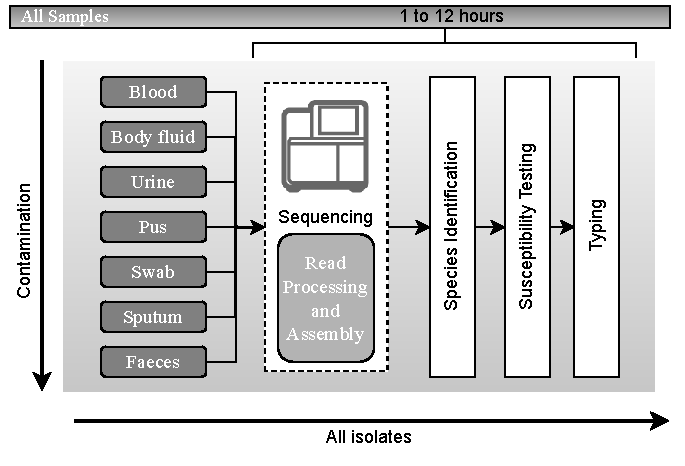
\includegraphics[width=\textwidth]{figures/introduction/Figure 4.pdf}
\caption{\textbf{Hypothetical workflow based on metagenomic sequencing.} Schematic representation of the hypothetical workflow for the direct processing of samples from suspected pathogen sources after adoption of metagenomic sequencing, with an expected timescale that could be accommodated in a single day. Adapted from \cite{didelot_transforming_2012}.}
\label{fig:figure4}
\end{figure*}


Albeit lacking consensus in the field, metagenomics can be classified into two variants as proposed by \citep{marchesi_vocabulary_2015}: (1) metaxonomics where marker genes ubiquitous in many taxa are targeted and sequenced, and (2) the untargeted "shotgun" sequencing of all microbial genomes present in a sample. 

\subsubsection{Metataxonomics and Targeted Metagenomics} \label{sssec:_intro_metataxonomics}

Molecular barcoding approaches can be combined with second-generation high-throughput sequencing to achieve unprecedented depths of coverage in microbial community profiling, being defined as metataxonomics. 
For profiling bacterial species, the most popular approach is 16S \ac{rRNA} gene sequencing, an ~1500 base pair gene that encodes catalytic RNA that is part of the 30S ribosomal subunit. 
Traditionally, the variable regions of the 16S \ac{rRNA} gene (V-regions) are targeted, or ranges thereof (V1-V2, V1-V3, V3-V4, V4, V4-V5, V6-V8, and V7-V9), and are specific to bacterial genus (96\%) and for some, even species (87.5\%), \citep{srinivasan_use_2015, abellan-schneyder_primer_2021}. 
Moreover, dedicated 16S databases that include near full-length sequences for a large number of strains and their taxonomic placements exist, such as RDP\footnote{\url{http://rdp.cme.msu.edu/}}, Greengenes\footnote{\url{https://greengenes.secondgenome.com/}}, silva\footnote{\url{https://www.arb-silva.de/}} and NCBI's 16S ribosomal RNA project\footnote{\url{https://www.ncbi.nlm.nih.gov/refseq/targetedloci/}} \citep{cole_ribosomal_2009, desantis_greengenes_2006, pruesse_silva_2007}. 
The sequence of an unknown strain can be compared with the sequences in these databases, after very closely related sequences are grouped into \ac{OTUs},  an operational definition used to classify groups of closely related individuals. This allows the deduction of probable taxonomy, with the assumption that sequences of $>$95\% identity represent the same genus, whereas sequences of $>$97\% identity represent the same species \citep{schloss_introducing_2005}. 

Furthermore, it must necessarily account for intragenomic variation between 16S gene copies. 
Furthermore, targeting 16S variable regions with short-read sequencing platforms cannot achieve the taxonomic resolution afforded by sequencing the entire gene and is limited by the database chosen \citep{johnson_evaluation_2019}. 
The emergence of third generating sequencing technologies (see \secref{ssec:_intro_3rd_gen_seq}) allows for this limitation to be overcome but currently, only a fraction of the databases includes complete 16S \ac{rRNA} sequences.

While viruses are an integral part of the microbiota, no universal viral marker genes are available to perform such taxonomic assignments. 
Amplification of whole viral genomes is possible and, in 2015, RNA extracted from whole blood, serum, re-suspended swabs and urine, after targeted amplification of the whole viral genome, proved invaluable in the track of the Ebola virus disease epidemic in West Africa, responsible for >11 thousand deaths, allowing for the characterisation of the infectious agent the determination of its evolutionary rate, signatures of host adaptation, identification and monitoring of diagnostic targets and responses to vaccines and treatments \citep{quick_real-time_2016}.
As an alternative, broad scope viral targeted sequence capture (TSC) panels offer depletion of background nucleic acids and improve the recovery of viral reads by targeting coding sequence from a multitude viral genera, such as VirCapSeq-VERT Capture Panel\footnote{\url{https://sequencing.roche.com/content/dam/rochesequence/worldwide/resources/brochure-vircapseq-vert-capture-panel-SEQ1000117.pdf}} but do not guarantee the full recovery of the viral genome, and can present biases towards certain genera \citep{schuele_assessment_2020, wylie_enhanced_2015}. 

\subsubsection{Shotgun Metagenomics} \label{sssec:_intro_shotgun_metagenomics}

\ac{SMg} can offer relatively unbiased pathogen detection and characterisation. The capacity to detect all potential pathogens — bacteria, viruses, fungi and parasites — in a sample has great potential utility in the diagnosis of infectious disease \citep{chiu_clinical_2019}, potentially able to provide genotyping, antimicrobial resistance and virulence profiling in a single methodological step. This comes with the cost of producing massive amounts of information that require expert handling and processing, as well as capable computational infrastructures \citep{couto_critical_2018, rossen_practical_2018}.

Clinical applications of \ac{SMg} derive its roots from the use of microarrays (see \secref{ssec:_intro_current_standards}), where it was successfully applied in in-depth microbiome analysis of different sites in the human body, it was the emergence of second-generation sequencing technology and its high throughput of genomic data at a competitive price that made sequencing of all genomic content, \ac{DNA} and/or RNA, in a clinical sample a viable possibility for diagnostics (see \secref{ssec:_intro_2nd_gen_seq} The second-generation of \ac{DNA} sequencing) \citep{miller_basic_2009, palmer_rapid_2006, chiu_clinical_2019}. The first reported case that demonstrated the utility of \ac{SMg} was in 2014 with the clinical diagnosis of neuroleptospirosis in a 14-year-old immunodeficient and critically ill boy with meningoencephalitis by Wilson et al \cite{wilson_actionable_2014}, prompting appropriate targeted antibiotic treatment and eventual recovery of the patient. In this case, traditional methods, including an invasive brain biopsy, failed to provide answers, until the shotgun sequencing of cerebrospinal fluid identified 475 of 3,063,784 sequence reads (0.016\%) corresponding to leptospira, for which clinical assays were negative due to its very low abundance. Ever since many other reports of successful application of \ac{SMg} in clinical metagenomics have been reported. but all in edge cases where traditional diagnostic methods have failed or as proof-of-concept \citep{couto_critical_2018, vijayvargiya_application_2019, sanabria_shotgun-metagenomics_2020, hirakata_application_2021}. 

In public health microbiology, \ac{SMg} combined with transmission network analysis allowed the investigation and quick action on the food supply of the 2013 outbreak of \ac{STEC} strain O104:H4 from faecal specimens obtained from patients \citep{loman_culture-independent_2013}. A similar approach was followed in the detection of \textit{Salmonella enterica} subsp. \textit{enterica} serovar Heidelberg from faecal samples in two though to be unrelated outbreaks in the United States of America, as well as the \textit{in situ} abundance and level of intrapopulation diversity of the pathogen, and the possibility of co-infections with \textit{Staphylococcus aureus}, overgrowth of commensal \textit{Escherichia coli}, and significant shifts in the gut microbiome during infection relative to reference healthy samples \citep{huang_metagenomics_2017}. More recently, shotgun metagenomic sequencing has evidenced alterations in the gut microbiota of a subset of COVID-19 patients that present the uncommon gastrointestinal (GI) symptoms, shedding a higher understanding of gut–lung axis affecting the progression of COVID-19 \citep{li_microbiome_2021}.

Clinical diagnostic applications have lagged behind research advances. A significant challenge with shotgun metagenomic approach is the large variation in the pathogen load between patient samples, as evidenced in the studies presented. A low pathogen load and  high contamination of host \ac{DNA} or even the present microbiome may result in enough data to produce the high-resolution subtype needed to distinguish and cluster the cases that were caused by the same outbreak pathogen source, or, extremely, the undetection of the causative agent \citep{carleton_metagenomic_2019, chiu_clinical_2019}. Differential lysis of human host cells followed by degradation of background \ac{DNA} has proven an effective method to reduce host contamination, but limitations include potential decreased sensitivity for microorganisms without cell walls, such as \textit{Mycoplasma} spp. or parasites; a possible paradoxical increase in exogenous background contamination by use of additional reagent \citep{salter_reagent_2014, oneil_ribosomal_2013, feehery_method_2013}. Additionally, it is often unclear whether a detected microorganism is a contaminant, coloniser or \textit{bona fide} pathogen, and the lack of golden standards remains one of the biggest challenges when applying these methods in clinical microbiology for diagnosis. 

In addition to negative controls, already a common practice in any sequencing assay and in particular in metataxonomics (see \secref{sssec:_intro_metataxonomics}), positive controls can be a way to circumvent the lack of golden standards, either through the spike of the samples with a known amount of a specific \ac{DNA}/RNA or though the sequencing of samples with known composition and abundance. Well-characterised reference standards and controls are needed to ensure the quality and stability of the \ac{SMg} assay over time \citep{chiu_clinical_2019, mcintyre_comprehensive_2017}. Most available metagenomic reference materials are highly tailored to a specific application. For example, the ZymoBIOMICS Microbial Community Standard\footnote{\url{https://www.zymoresearch.com/collections/zymobiomics-microbial-community-standards}} is the first commercially available standard for microbiomics and metagenomics studies, providing mock a mock community with defined composition and abundance consisting of Gram-positive, Gram-negative and yeast. It is useful to determine the limit of detection of an assay, and the effectiveness and biases of a given protocol. Standards with a more limited spectrum of organisms are also available, such as the \ac{NIST}\footnote{\url{https://www.nist.gov/}} reference materials for mixed microbial \ac{DNA} detection, which contain only bacteria. Thus, these materials may not apply to untargeted \ac{SMg} analyses.

\section{The role of bioinformatics} \label{sec:_intro_bioinformatics}

As stated previously (see \secref{sec:_intro_genomics_approach} and \secref{ssec:_intro_metagenomics}), one of the biggest challenges when dealing with genomic, and in particular metagenomic, data is the lack of golden standards. This is also applicable to the bioinformatic analysis, required due to the amount of data produced by genomic sequencing technologies. This is currently one of the bottlenecks in the deployment of sequencing technology in clinical microbiology as there is no standard in how to deal with the increasing amount of data produced in a fit-for-purpose manner \citep{carrico_primer_2018}.

Bioinformatics is an interdisciplinary research field that applies methodologies from computer science, applied mathematics and statistics to the study of biological phenomena\citep{carrico_primer_2018}. With the widespread use and continuous development of sequencing technologies, bioinformatics has become a cornerstone in modern clinical microbiology. 
Major efforts are being made on the standardisation and assessment of software for the analysis of genomic data, both commercial and open-source \cite{angers-loustau_challenges_2018, gruening_recommendations_2019, sczyrba_critical_2017, couto_critical_2018}. 

\subsection{From molecules to reads}

In all sequencing technologies (see \secref{ssec:_intro_sequencing}), many copies of the source \ac{DNA} are randomly fragmented and sequenced. To these sequences, we refer to as reads. In the case of second-generation sequencing (see \secref{ssec:_intro_2nd_gen_seq} The second-generation of \ac{DNA} sequencing), one or both ends of the fragment can be sequenced. If a fragment is sequenced from one end, we refer to it as single-end sequencing. If a fragment is sequenced on both ends, spanning the entire fragment, it is called paired-end sequencing.

\subsubsection{The FASTQ file} \label{sssec:_intro_fastq}

All sequencing technologies, regardless of generation, produce data in the same standard file format: the FASTQ, a text-based format for storing both a biological sequence (usually nucleotide sequence) and its corresponding quality scores \citep{cock_sanger_2010}. Originally developed at the Wellcome Trust Sanger Institute, the FASTQ has emerged as a common file format for sharing sequencing read data (see \ref{fig:figure3}). The FASTQ can be considered as an extension of the ‘FASTA sequence file format’, originally invented by \cite{pearson_improved_1988}, which includes just the sequence information. A FASTQ file normally uses four lines per sequence:

\begin{itemize}
    \item \textbf{Line 1} begins with a '@' character and is followed by a sequence identifier and an optional description;
    \item \textbf{Line 2} is the raw sequence letters;
    \item \textbf{Line 3} begins with a '+' character and is optionally followed by the same sequence identifier (and any description) again;
    \item \textbf{Line 4} encodes the quality values for the sequence in Line 2, and must contain the same number of symbols as letters in the sequence.
\end{itemize}

In FASTQ both the sequence letter and quality score are each encoded with a single ASCII character for brevity. The quality of a sequence in a FASTQ file is represented by a quality value Q is an integer mapping of p, where p is the probability that the corresponding base call is incorrect (see Table \ref{tab:phred_error}). This is called the PHRED score \citep{ewing_base-calling_1998} and is defined by the following equation:

\begin{equation}
\centering
\mathbf{Q}\textsc{phred} = - 10 \times \log \mathbf{P}
\end{equation}
 
The PHRED quality scores $\mathbf{Q}$ is defined as a property which is logarithmically related to the base-calling error probability $\mathbf{P}$.

\begin{table}[h!]
\caption{\textbf{PHRED quality scores are logarithmically linked to error probabilities.} A PHRED Score of 20 indicates the likelihood of finding 1 incorrect base call among 100 bases. In other words, the precision of the base call is 99\%. $\mathbf{Q}$ scores are classified as a property that is associated logarithmically with the probabilities of base calling error $\mathbf{P}$.} \label{tab:phred_error}
\resizebox{\textwidth}{!}{%
\begin{tabular}{@{}lll@{}}
\toprule
\textbf{Phred Quality Score} & \textbf{Probability of incorrect base call} & \textbf{Base call accuracy} \\ \midrule
10 & 1 in 10        & 90\%     \\
20 & 1 in 100       & 99\%     \\
30 & 1 in 1000      & 99.90\%  \\
40 & 1 in 10,000    & 99.99\%  \\
50 & 1 in 100,000   & 100.00\% \\
60 & 1 in 1,000,000 & 100.00\% \\ \bottomrule
\end{tabular}%
}
\end{table}

Since their introduction, PHRED scores have become the \textit{de facto} standard for representing sequencing read base qualities \citep{cock_sanger_2010}. Despite this convention, the encoding of the Phread score can vary when translated to its ASCII representation in the FASTQ file format. For example, Sanger FASTQ files use ASCII 33–126 to encode PHRED qualities from 0 to 93 (that is, PHRED scores with an ASCII offset of 33). A full list of encoding is available in Figure \ref{fig:figure6}. 

\begin{figure*}[h!]
\centering
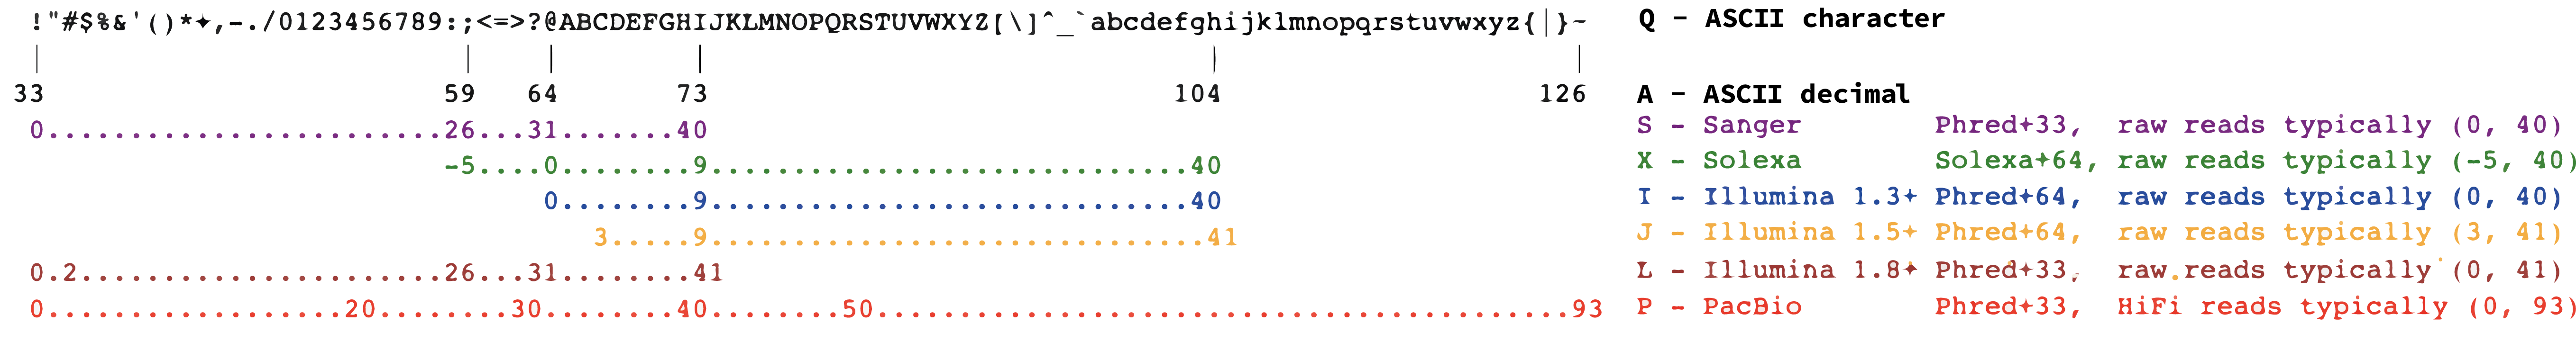
\includegraphics[width=\textwidth]{figures/introduction/Figure 6.png}
\caption{\textbf{Range of FASTQ quality scores and their corresponding ASCII encoding.} For raw reads, the range of scores will depend on the technology and the base caller used. Starting in Illumina 1.8, the quality scores have returned to the use of the Sanger format (PHRED+33). For processed reads and long accurate reads, scores may be even higher with, for example, quality values of up to 93 observed in reads from PacBio HiFi reads.}
\label{fig:figure6}
\end{figure*}

\subsubsection{FASTQ file simulation} \label{ssec:_intro_fastq_sim}

With the lack of golden standards for metagenomic analysis, the use of simulated mock communities, with known composition, abundance, and genomic information, provides a ground truth against which success evaluations can be made. Given their standard structure and adoption, the generation of simulated FASTQ files from a reference or a set of references is very straightforward. 

Multiple computational tools have been developed in recent years for the simulation of sequencing data, particularly for second and third-generation sequencing technologies, which could be used to compare existing and new bioinformatic analytical pipelines. \cite{escalona_comparison_2016} provides a comprehensive assessment of 23 different read-simulation tools,  highlighting their distinct functionality, requirements, and potential applications, as well as providing a selection of suggestions for different simulation tools depending on their purpose. For \textit{in silico} genomic and metagenomic sequence generation, a plethora of tools are available for first, second and third-generation reads (see Figure \ref{fig:figure7}).

\begin{figure*}[h!]
\centering
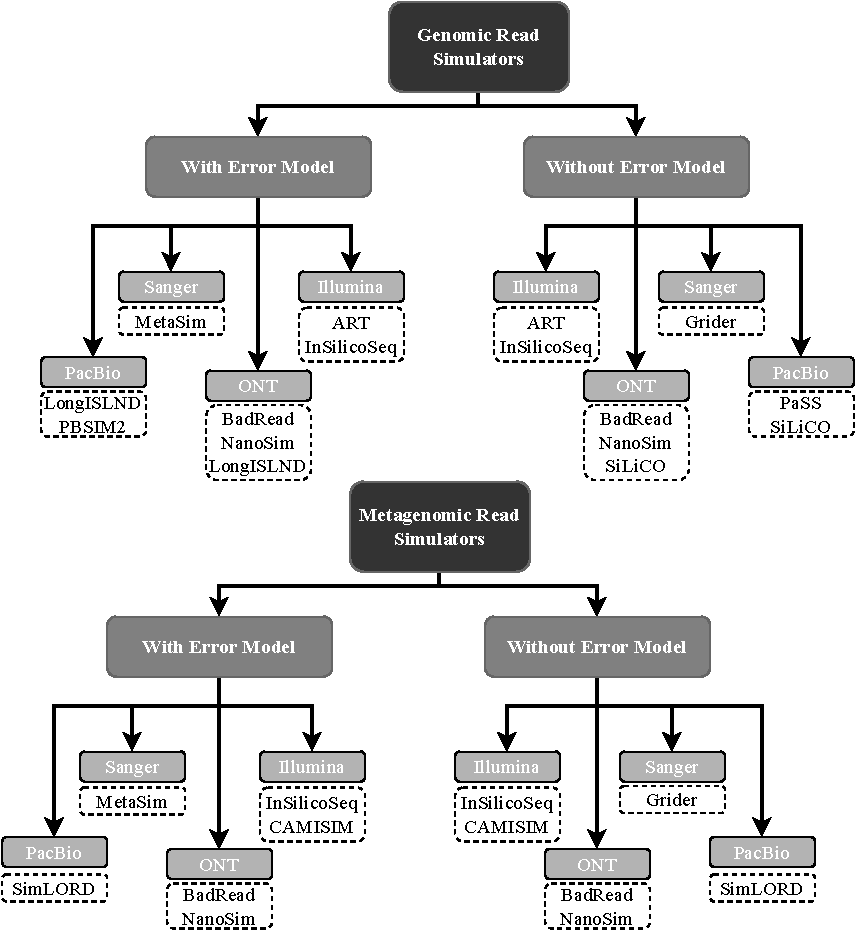
\includegraphics[width=\textwidth]{figures/introduction/Figure 7.pdf}
\caption{\textbf{Sequence simulators for genomic and metagenomic data.} For first generation sequencing, Metasim (\url{https://github.com/gwcbi/metagenomics_simulation}) and Grider (\url{https://sourceforge.net/projects/biogrinder/}) can generate mock genomic and metagenomic data, with and without error models, respectively. For Illumina data, ART (\url{https://www.niehs.nih.gov/research/resources/software/biostatistics/art/index.cfm}), InSilicoSeq (\url{https://github.com/HadrienG/InSilicoSeq}) and CAMISIM (\url{https://github.com/CAMI-challenge/CAMISIM}) represent options for in silico data generation. Due to their differences, the third-generation \ac{PacBio} and Oxford Nanopore (ONT) have distict software for in silico data generation. The first can be accomplished by LongISLND (\url{https://bioinform.github.io/longislnd/}) and PBSIM2 (\url{https://github.com/yukiteruono/pbsim2}) got genomic data, and SimLORD (\url{https://bitbucket.org/genomeinformatics/simlord/src}) fot metagenomic data, with and without error model. The latter BadRead (\url{https://github.com/rrwick/Badread}) and NanoSim (\url{https://github.com/bcgsc/NanoSim}) can genenrate genomic and metagenomic \textit{in silico} data, with and withouth error model. Additionally, for genomic data, LongISLND and SiLiCO (\url{https://github.com/ethanagb/SiLiCO}) generate data with and without error, respectively. Adapted from \cite{escalona_comparison_2016}.}
\label{fig:figure7}
\end{figure*}

\subsubsection{FASTQ quality assessment and quality control} \label{ssec:_intro_fastq_quality}

Quality assessment and control is a basal step to any analysis, and aims to (1) remove and/or filter low quality and low complexity reads, (2) trim adapters, and (3) remove host sequences from the samples’ raw data. There are many tools available but the most commonly used are FastQC\footnote{\url{https://www.bioinformatics.babraham.ac.uk/projects/fastqc/}} (Babraham Bioinformatics) for quality control, followed by Trimmomatic \citep{bolger_trimmomatic_2014}, Cutadapt \citep{martin_cutadapt_2011} or fastp \citep{chen_fastp_2018} to trim and/or filter adaptors, low quality and low complexity sequences. For long-read sequencing, tools like NanoPlot and NanoStats \citep{de_coster_nanopack_2018}, and Filtlong\footnote{\url{https://github.com/rrwick/Filtlong/}} can perform the equivalent quality assessment and control, adapter trimming and low quality trimming, respectively. 

\subsubsection{Direct taxonomic assignment and characterisation} \label{sssec:_intro_taxonomic_assignment}

A piece of important information that can be retrieved directly from the quality-controlled read data: (1) the identification and characterisation of the microbes present in a sample and (2) their relative abundance. Taxonomic classification methods can vary depending on the sequencing methodology used: pure culture, metataxonomics and amplicon metagenomics, and shotgun metagenomics.

From pure culture, taxonomic identification of the read content of a sample is useful to assess contamination. Tools like Kraken2 \citep{wood_kraken_2014, wood_improved_2019} and Braken \citep{lu_bracken_2017}. These tools, relying on a database, assign taxonomic labels to reads and are therefore biased to the contents of the database used. Various databases are available\footnote{\url{https://benlangmead.github.io/aws-indexes/k2}}, varying in size and content (archaea, bacteria, viral, plasmid, human and eukaryotic pathogens) and therefore in sensitivity depending on the resources available and the purpose intended. Alternatively, there are options to create custom databases.  

These tools are also extremely useful to assess the contents of a metagenomic sample. Alternatives such as Midas \citep{nayfach_integrated_2016}, Kaiju, \citep{menzel_fast_2016}, and MetaPhlAn2 \citep{truong_metaphlan2_2015} offer the same analysis as Kraken and Bracken using different algorithms, and with the disadvantage that they come prepackaged with their own databases, without the option to create a tailored database, limiting their applicability. Kaiju differs from the other tools by using a protein reference database, instead of nucleotide, but no pre-built version is available, requiring significant resources to build and index the database pre-use. Long-read data from third-generation sequencing technologies (see \secref{ssec:_intro_3rd_gen_seq}) can be treated as single-end reads, and all mentioned tools accommodate the classification of single-end files. 

\subsection{From reads to genomes} \label{ssec:_intro_reads_2_genomes}

Due to the limitations of current sequencing technologies (see \secref{ssec:_intro_sequencing}), the order of the reads produced by these machines cannot be preserved. 
Therefore, to obtain the true original genomic sequence the process of "genome assembly" has to occur, where FASTQ files, containing the sequencing information, are converted into FASTA files with informative genomic sequences. Information can be inferred through genome annotation software, such as Prokka\footnote{\url{https://github.com/tseemann/prokka}}, identifying and labelling all relevant features in a genome sequence, such as predicted coding regions and their putative products, noncoding RNAs, signal peptides, and so on \citep{seemann_prokka_2014}. 


The term "draft genome" is commonly used because these sequencing technologies do not generate a single closed genome, particularly short-read such as in second generation sequencing (see \secref{ssec:_intro_2nd_gen_seq} The second-generation of DNA sequencing) which need to be assembled into usually a series of sequences (contigs) that may cover up to 95\% to 99\% of the strain genome \citep{carrico_primer_2018}. 
Long-read technologies (see \secref{ssec:_intro_3rd_gen_seq}) allow for this value to reach 100\%, effectively producing closed, complete genomes, notwithstanding that this value can sometimes overcome the 100\% due to overlap \citep{wick_benchmarking_2021}.

Assembling reads into contigs has many advantages, namely that longer sequences are more informative, allowing the consideration of whole genes or even gene clusters within a genome and to understand larger genetic variants and repeats. Additionally, it has the effect of removing most sequencing errors, though this can be at the expense of new assembly errors \citep{ayling_new_2020}. Two methods are used to obtain draft genomes: (1) through reference-guided sequence assembly, or (2), through \textit{de novo} sequence assembly.

\subsubsection{The FASTA file} \label{sssec:_intro_fastq}

In bioinformatics, the FASTA format is a text-based format to represent nucleotide or amino acid sequences using single-letter codes, preceded by a sequence name or any other information relative to the sequence. Similarly to FASTQ (see \ref{ssec:_intro_fastq}), it was developed by the Wellcome Trust Sanger Institute, the FASTQ has emerged as a common file format for sharing sequence data \citep{pearson_improved_1988}. The FASTA file follows the following conformation:

\begin{itemize}
    \item The \textbf{first line} of a FASTA file starts with a ">" (greater-than) symbol, signifying the comment portion;
    \item The \textbf{subsequent lines} containing the actual sequence itself represented in the standard IUB/IUPAC amino acid and nucleic acid codes \citep{e_iupac-iub_1970}, usually 80 characters in length.
\end{itemize}

A multiple sequence FASTA format can be obtained by concatenating several single sequence FASTA files in a common file (also known as multi-FASTA format). The extension of the file indicates the type of sequence (nucleotide or amino acid) present (see Table \ref{tab:fasta_extension}). For genomic data, the ".fasta", ".fa", ".fna", and ".ffn" are the most used, with the first two being generic and the last two specific for nucleic acid and coding regions of a genome. 

\begin{table}[h!]
\caption{The standard filename extension for a text file containing FASTA formatted sequences.}
\label{tab:fasta_extension}
\resizebox{\textwidth}{!}{%
\begin{tabular}{@{}lll@{}}
\toprule
\textbf{Extension} & \textbf{Sequence}                         & \textbf{Definition}                                                                    \\ \midrule
fasta, fa & generic FASTA                    & Any generic fasta file. See below for other common FASTA file extensions      \\ 
fna       & FASTA nucleic acid               & Used generically to specify nucleic acids.                                    \\
ffn       & FASTA nucleotide of gene regions & Contains coding regions for a genome.                                         \\
faa & FASTA amino acid & Contains amino acid sequences. A multiple protein fasta file can have the more specific extension mpfa. \\
frn       & FASTA non-coding RNA             & Contains non-coding RNA regions for a genome, in DNA alphabet e.g. tRNA, rRNA \\ \bottomrule
\end{tabular}%
}
\end{table}

\subsubsection{Genomes through reference-guided sequence assembly}

A reference-guided genome assembly uses an already sequenced reference genome to assemble a new genome, making use of the similarity between target and reference species to gain additional information, which often lead to a more complete and improved genome \citep{rausch_consistency-based_2009, lischer_reference-guided_2017}. 
This process is usually done through the mapping of the reads to a closely related reference sequence, and as more and more species get sequenced, the chances that a genome of the same or related species is already available, in which a significant proportion of the reads can be mapped, increase greatly. 
This process usually includes the following steps: (1) the reference genome has to be indexed, allowing compression of the input text while still permitting fast sub-string queries, (2) for each short-read several sub sequences (seeds) are taken and searched to find their exact matches in the reference  (candidate regions), (3) each short-read is then aligned to all corresponding candidate regions, and (4) the consensus sequence is computed in which the reference sequence is corrected when there is enough evidence of an difference based on the mapped
reads, identifying the differences between it and the newly generated consensus sequence \citep{bayat_methods_2020}.
In addition to variants, the new consensus genome might have insertions or deletions with respect to the reference genome.

Besides the generation of a consensus sequence, the mapping of the reads to the reference sequence can be used to estimate sequence depth and breadth of coverage. 
Depth of coverage, often referred to simply as coverage, refers to the average number of times each nucleotide position in the strain's genome has a read that aligns to that position. Depending on the study goals, bacterial species, and the intended analyses, the optimal depth of coverage varies. 
In public repositories, most submissions have a depth of coverage ranging from 15 to 500 times \citep{carrico_primer_2018}. 
The breadth of coverage is defined as the ratio of covered sequence on the reference by aligned reads.

\subsubsection{Genomes through \textit{de novo} sequence assembly}

The \textit{de novo} assembly refers to the bioinformatics process whereby reads are assembled into a draft genome using only the sequence information of the reads. Two methods are used to obtain draft genomes without the need of a reference genome: (1) through Overlap, Layout and Consensus, or (2) De Bruijn graph assembly (see Figure \ref{fig:figure8}). The \textit{de novo} assembly methods provide longer sequences that are more informative than shorter sequencing data and can provide a more complete picture of the microbial community in a given sample.

\begin{figure*}[h!]
\centering
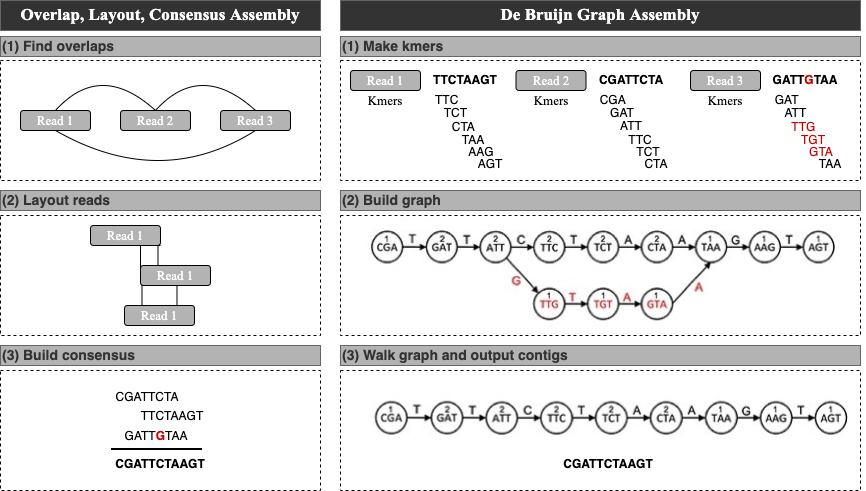
\includegraphics[width=\textwidth]{figures/introduction/Figure 8.png}
\caption{\textbf{Approaches to \textit{de novo} genome assemble.} In Overlap, Layout, Consensus assembly, (1) overlaps are found between reads and an overlap graph constructed (edges indicate overlapping reads). (2) Reads are laid out into contigs based on the overlaps (lines indicate overlapping portions). (3) The most likely sequence is chosen to construct consensus sequence. In the De Bruijn graph assembly, (1) reads are decomposed into kmers of a determined size by sliding a window of size k (in here of k=3) across the reads. (2) The kmers become vertices in the De Bruijn graph, with edges connecting overlapping kmers. Polymorphisms (red) form branches in the graph. A count is kept of how many times a kmer is seen, shown here as the numbers above kmers. (3) Contigs are built by walking the graph from the edge nodes. A variety of heuristics handle branches in the graphs—for example, low coverage paths, as shown here, may be ignored. Adapted from \cite{ayling_new_2020}}.
\label{fig:figure8}
\end{figure*}

\paragraph{Overlap, Layout and Consensus assembly} \label{sssec:_intro_OLC_assembly} \mbox\\

First-generation sequencing technology (see \secref{ssec:_intro_1st_gen_seq}) produces far fewer reads than second-generation sequencing technology (see \secref{ssec:_intro_2nd_gen_seq} The second-generation of DNA sequencing), but individual reads are longer (500 to 1000 \ac{bp}). 
Assembly of Sanger data usually uses \ac{OLC} approaches, in which:

\begin{itemize}
    \item Overlaps are computed by comparing all reads to all other reads;
    \item Overlaps are grouped together to form contigs;
    \item A consensus contiguous sequence, or contig, is determined by picking the most likely nucleotides from the overlapping reads.
\end{itemize}

These types of assemblers were very popular in the early 2010s, with assemblers such as Celera\footnote{\url{https://www.cbcb.umd.edu/software/celera-assembler}},  Genovo\footnote{\url{https://cs.stanford.edu/genovo }}, xGenovo\footnote{\url{http://xgenovo.dna.bio.keio.ac.jp/}} and BBAP\footnote{\url{http://homepage.ntu.edu.tw/~youylin/BBAP.html}} having been widely used \citep{myers_whole-genome_2000, hutchison_genovo_2010, afiahayati_extended_2013, lin_novo_2017}.
With the emergence of third-generation sequencing (see \secref{ssec:_intro_3rd_gen_seq} The third-generation of DNA sequencing), \ac{OLC} assemblers have been increasingly developed and adopted by the community to assembly long-read data. 
In the latest years, ra\footnote{\url{https://github.com/lbcb-sci/ra}}, raven\footnote{\url{https://github.com/lbcb-sci/raven}} and canu\footnote{\url{https://github.com/marbl/canu}}, the latter being a a fork of the Celera Assembler, have become staples in the community, showing good reliability and amassing over 3000 citations \citep{vaser_yet_2019, koren_canu_2017, wick_benchmarking_2021}.

\paragraph{De Bruijn graph assembly} \label{sssec:_intro_dbg_assembly} \mbox{}\\

In the De Bruijn assembly graph, reads are split into overlapping k-mers where nodes of the graph represent k-mers where:

\begin{itemize}
    \item A directed edge from node N\textsubscript{a} to node N\textsubscript{b} indicates that N\textsubscript{b} is next to N\textsubscript{a} in a read;
    \item The number of nodes in the De Bruijn graph is theoretically the total number of identical k-mers in the genome;
    \item The weight on the edge indicates the number of times N\textsubscript{b} is observed next to N\textsubscript{a} in all reads.
\end{itemize}

Thus, the weight of an edge indicates the possibility that two k-mers appear after each other in the \ac{DNA} sequence. A path in the graph where all edges have the highest weight is the most likely to be a part of the genome \citep{bayat_methods_2020}.

Most second-generation sequencing (see \secref{ssec:_intro_2nd_gen_seq} The second-generation of \ac{DNA} sequencing) assemblers, such as SPAdes\footnote{\url{https://github.com/ablab/spades/}} and  SKESA\footnote{\url{https://github.com/ncbi/SKESA/}}, use a multiple k-mer De Bruijn graph, starting with the lowest size and iteratively adding k-mers of increasing length to connect the graph \citep{bankevich_spades_2012, souvorov_skesa_2018, li_megahit_2015}. Older assemblers, such as Velvet\footnote{\url{https://www.ebi.ac.uk/~zerbino/velvet/}}, Ray\footnote{\url{https://sourceforge.net/projects/denovoassembler/f}} and SoapDeNovo2\footnote{\url{https://sourceforge.net/projects/soapdenovo2/}} use a single k-mer strategy for the De Bruijn graph construction \citep{zerbino_velvet_2008, boisvert_ray_2010, luo_soapdenovo2_2012}. 

\subsubsection{Assembly quality assessment and quality control} \label{ssec:_intro_assembly_quality}

The success of an assembly is evaluated in two steps: (1) globally, through intrinsic characteristics of the assembly itself, and (2) relative to a reference genome. The computation of the global metrics is performed through statistics inherent to the complete set of contigs assembled per sample, independent of the species/sample of origin. Commonly, these statistics include information on contig number, its median size and number ambiguous bases. The comparison with a reference sequence allows statistics such as the number of misassemblies, meaning contigs that do not reflect the structural organisation in the reference sequence, to be computed. 

Assessment and evaluation of genome assemblies has been a relevant field ever since the emergence of the assembly process itself. 
The most widely adopted is QUAST\footnote{\url{http://quast.sourceforge.net/quast}}, can evaluate assemblies both with a reference genome, as well as without a reference, producing many reports, summary tables and plots to help compare and assess assembly success \citep{gurevich_quast_2013}, but alternatives, such as GenomeQC\footnote{\url{https://github.com/HuffordLab/GenomeQC}} exist \citep{manchanda_genomeqc_2020}. 

\subsection{Reproducibility, replicability and transparency} \label{ssec:_intro_reproducibility}

Computational algorithms have become an essential component of microbiome research, with great efforts by the scientific community to raise standards on the development and distribution of code. A lack of reproducibility in computational biology research can be attributed to many factors such as an incomplete or erroneous descriptions of the software used, incomplete documentation on how to run an analysis, or failing to make available the relevant computer code needed \citep{papin_improving_2020}.  As early as 1990, movements for reproducible research, with special focus on computation-intensive scientific work, have arisen, brought on by the growing use of computational workflows for analysing data across a range of disciplines \citep{claerbout_electronic_1992}

Despite the presented efforts, the effectiveness in computational reproducibility is still questionable. Stodden et al \citep{stodden_empirical_2018} reported that, in 22 randomly selected publications who's results relied on the use of computational and data-enabled methods and deemed to be reproducible (i.e. provided data and/or code), only 14\% were straightforward to reproduce with minimal effort. Similar results have been observed in comparable studies \citep{baggerly_deriving_2009, kim_experimenting_2018, huang_comparability_2013}

Several steps can be implemented to ensure the transparency and reproducibility of the chosen bioinformatic workflow. Despite these efforts, sustainability and reproducibility are still major issues. In the field of microbial bioinformatics are not yet widely adopted. The FAIR Principles, standing for Findability, Accessibility, Interoperability, and Reusability, put specific emphasis on enhancing the ability to find and reuse not only data but also the algorithms, tools, and workflows that led to that data \citep{wilkinson_fair_2016}. The FAIR guiding principles can be summarised as follows:

\begin{itemize}
    \item \textbf{To be Findable:}
    \begin{itemize}
        \item F1. (meta)data are assigned a globally unique and persistent identifier
        \item F2. data are described with rich metadata (defined by R1 below)
        \item F3. metadata clearly and explicitly include the identifier of the data it describes
        \item F4. (meta)data are registered or indexed in a searchable resource
    \end{itemize}
    \item \textbf{To be Accessible:}
    \begin{itemize}
        \item A1. (meta)data are retrievable by their identifier using a standardised communications protocol
        \begin{itemize}
            \item A1.1 the protocol is open, free, and universally implementable
            \item A1.2 the protocol allows for an authentication and authorisation procedure, where necessary
        \end{itemize}
        \item A2. metadata are accessible, even when the data are no longer available
    \end{itemize}
    \item \textbf{To be Interoperable:}
    \begin{itemize}
        \item I1. (meta)data use a formal, accessible, shared, and broadly applicable language for knowledge representation.
        \item I2. (meta)data use vocabularies that follow FAIR principles
        \item I3. (meta)data include qualified references to other (meta)data
    \end{itemize}
    \item \textbf{To be Reusable:}
    \begin{itemize}
        \item R1. meta(data) are richly described with a plurality of accurate and relevant attributes
        \item R1.1. (meta)data are released with a clear and accessible data usage license
        \item R1.2. (meta)data are associated with detailed provenance
        \item R1.3. (meta)data meet domain-relevant community standards
    \end{itemize}
\end{itemize}

Several steps have been recommended by experts to ensure the FAIR'ness of both software and data \citep{ram_git_2013, piccolo_tools_2016, boettiger_introduction_2015, sandve_ten_2013}. Favouring open-source tools, with clear documentation describing the methodology implemented and stating the version of the software used and which parameters were used, enables the comparison of results. 
This can be simplified by containerising all software tools with one of the many available solutions, such as Docker\footnote{\url{https://www.docker.com/}} or Singularity\footnote{\url{https://sylabs.io/}} \citep{kurtzer_singularity_2017}. The use of workflow managers, like nextflow\footnote{\url{https://www.nextflow.io/}}, snakemake\footnote{\url{https://snakemake.github.io/}} or the Galaxy Project\footnote{\url{https://galaxyproject.org/}}, will push reproducibility to the next level by taking advantage of the containerisation and scalability, enabling the workflow to be executed with the same parameters in the same conditions in a multitude of different environments \citep{di_tommaso_nextflow_2017, molder_sustainable_2021, afgan_galaxy_2018}. 

When developing software, in the field of microbial bioinformatics, good software engineering practices are not yet widely adopted. An example of such is the widespread use of \ac{VSC}, which have long been used to maintain code repositories in the software industry, are now finding new applications in science \citep{ram_git_2013}. Git\footnote{\url{https://git-scm.com/}}, a free and open source distributed version control system designed to handle everything from small to very large projects with speed and efficiency,  provides a powerful way to track and compare versions, retrace errors, explore new approaches in a structured manner, while maintaining a full audit trail. Remote \ac{VSC} hosting services, such as GitHub\footnote{\url{https://github.com/}}, allows for this functionality to be expanded by placing the software in a central location so that it can be accessed by multiple developers and users, facilitating collaboration and auditability. Another example is the use of continued validation through software testing. Modern software engineering advocates reliable software testing standards and best practices. Different approaches are employed: from unit testing to system testing, going from testing every individual component to testing a tool as a whole, verifying and demonstrating that that the published code and data are working properly \citep{krafczyk_scientific_2019}.

\section{Bioinformatic Analysis for Metagenomics} \label{sec:_intro_metagenomics_bioinfo}

As mentioned previously (see \secref{ssec:_intro_metagenomics}, Metagenomic shotgun sequencing circumvents the need for cultivation and, compared with metataxonomics, avoids biases from primer choice, enables the detection of organisms across all domains of life and \textit{de novo} assembly of genomes and functional genome analyses. However, highly uneven sequencing depth of different organisms and low depth of coverage per species are drawbacks that limit taxa

\subsubsection{Metataxonomics} \label{ssec:_intro_metataxonomics_bioinfo}

Metataxonomics (see \secref{sssec:_intro_metataxonomics}) is the most widely used technique for microbial diversity analysis \citep{hilton_metataxonomic_2016}, and due to its particularities, the analysis of this data is also very particular. Data analyses are mostly carried out through specialised pipelines that wrap and combine several tools, offering the possibility to follow a simple protocol with default configurations or choose between a plethora of different configurations to adjust for any particular needs. Quantitative Insights Into Microbial Ecology 2 (QUIIME2)\footnote{\url{https://qiime2.org/}} \citep{bolyen_reproducible_2019} has become the \textit{de facto} tool for metataxonomic analysis as a framework with an ever-growing suite of plugins and intuitive data visualisation tools for the assessment of results. Mothur \citep{schloss_introducing_2009} and UPARSE \citep{edgar_uparse_2013} are also a popular alternative although resulting outputs differing significantly between pipelines despite using the same inputs having been reported by \cite{marizzoni_comparison_2020}, with a magnitude that is comparable to differences in upstream sample treatment and sequencing procedures.  A typical workflow starts with quality filtering, error correction and removal of chimeric sequences. These quality control steps are followed by either taxonomic assignment of reads or a clustering step where reads are gathered into \ac{OTUs} given their sequence identity, followed by statistical analysis to assess differences between given groups. Taxonomic assignment methods classify query sequences based on the best hit found in reference databases of annotated sequences, being heavily dependent on the completeness of the reference databases (see \secref{sssec:_intro_metataxonomics}). Classification is further limited by lack of species annotation in most reference databases \citep{westcott_novo_2015}. Alternatively, the same approach of direct taxonomic classification, without \ac{OTUs} clustering, can be followed as with genomic and shotgun metagenomic data, given that the databases include \ac{rRNA} sequences.

\ac{OTUs} clustering methods can be categorised into: (1) computationally expensive hierarchical methods that cluster sequences based on a distance matrix measuring the difference between each pair of sequences, (2) less expensive heuristic methods cluster sequences into \ac{OTUs} based on a pre-defined threshold, generally, with a sequence being selected as a seed and the rest of the sequences being analysed sequentially and added to existing or new clusters according to the defined threshold, and (3) model based clustering methods that do not rely on a pre-defined and fixed threshold, defining \ac{OTUs} based on a soft threshold and carrying out the clustering process based on methods such as an unsupervised probabilistic Bayesian clustering algorithm \citep{hao_clustering_2011}. These methods offer the possibility to cluster sequences based on criteria that do not depend on reference databases and are especially useful in less characterised microbial communities or with a high representation of uncultured microbes. Due to the assumptions made with this strategy, it is sensitive to under or overestimation of the number of \ac{OTUs} in a sample as defining a threshold to accurately cluster sequences is difficult \citep{westcott_novo_2015}.

\subsubsection{Shotgun metagenomics} \label{ssec:_intro_shotgun_metagenomics_bioinfo}

A plethora of open-source tools are available specifically for shotgun metagenomic data, and several combinations of these tools can be used to characterise the causative agent in a patient's infection in a fraction of the time required by the traditional methods. 

A major additional difficulty of shotgun metagenomic data is the overpowering quantities of host \ac{DNA} that are often sequenced, making the microbial community sometimes close to undetectable \citep{couto_critical_2018}.
The presence of contaminants, from the bench process to the pre-existing biota, and the cost associated with this methodology, are also major hinders in its applicability in the clinic.
They account for major caveats and must be made aware of when analysing the data.

\begin{figure*}[h!]
\centering
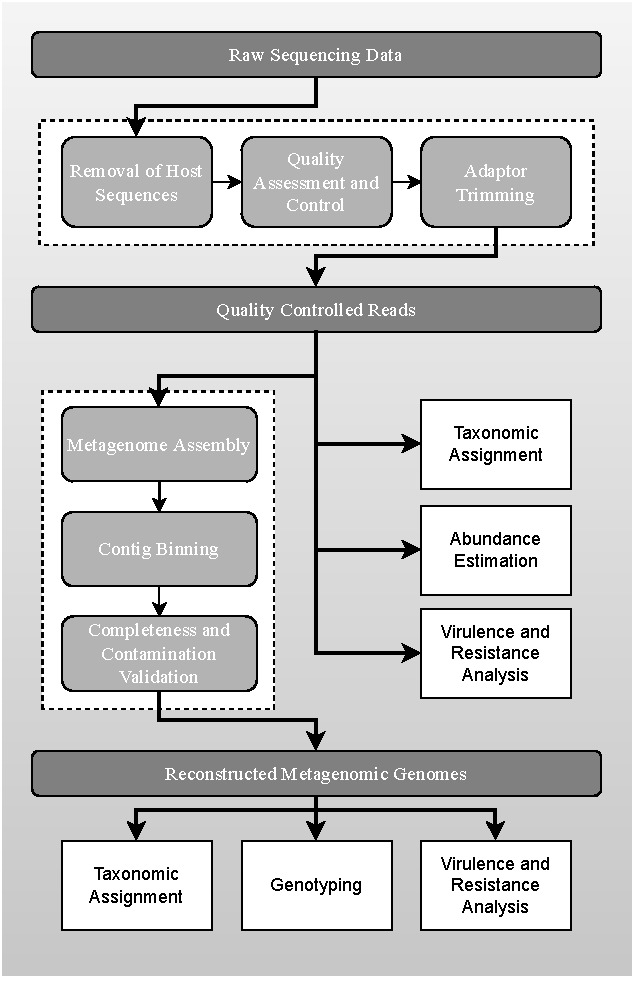
\includegraphics[]{figures/introduction/Figure9.pdf}
\caption{Typical bioinformatic analysis procedure for metagenomic data}
\label{fig:figure9}
\end{figure*}

The basic strategies for analysing shotgun metagenomic data can be simplified in the scheme in Figure \ref{fig:figure9}. 
One of the biggest challenges when doing metagenomic analysis is differentiating between colonisation and infection by successfully discriminating between a potential pathogen and background microbiota. 
In the latter, when analysing samples from presumably sterile sites, like cerebrospinal fluid and blood, it is safe to assume that all organisms found are of interest. 
In locations with a microbiota, the inclusion of negative controls is essential for the correct identification of contaminants in the taxonomic results, whether originated from the sample collection, handling or sequencing process. 
The use of spiked metagenomic samples as positive control might guide the detection of the possible pathogens by comparing relative abundance between the samples. 
These controls should be processed similarly to the samples and the taxonomic results should be filtered out from the final report. 

As explored in \secref{ssec:_intro_reads_2_genomes}, longer sequences are more informative than shorter sequencing data, as the one obtained from second-generation sequencing (see \secref{ssec:_intro_2nd_gen_seq} The second-generation of \ac{DNA} sequencing), and can provide a more complete picture of the microbial community in a given samples. 
Several dedicated metagenomic assembly tools are available, such as metaSPAdes\footnote{\url{https://github.com/ablab/spades/}}  and MegaHIT\footnote{\url{https://github.com/voutcn/megahit/}} \citep{nurk_metaspades_2017, li_megahit_2015}. 
These tools, in comparison to single-cell data assemblers, are better at dealing with the combination of intra and intergenomic repeats and uneven sequencing coverage \citep{olson_metagenomic_2017}.
For third-generation sequencing, dedicated metagenomic assemblers have recently emerged, such as meta-flye\footnote{\url{https://github.com/fenderglass/Flye/}} which expands on the original flye assembler by overcoming a k-mer selection limitation on low abundance species \citep{kolmogorov_metaflye_2020}. Nevertheless, the use of non dedicated assemblers for metagenomics may come with the cost of wrongly interpret variation as error, especially in samples that contained closely related species and the construction of chimeric sequences as traditional assemblers follow the basic principle that the coverage in a sample is constant \citep{teeling_current_2012}. 

The assembly-based approach requires the grouping of the different contigs into bins, ideally each collecting the sequences that belong to a microorganism present in the sample. The binning process can be taxonomy dependent, relying on a database to aggregate the sequences, or independent. The independent approach has the benefit of not relying on a database, but instead it uses the composition of each sequence and coverage profiles to cluster together sequences that might belong to the same organism. These algorithms don’t require prior knowledge about the genomes in a given sample, instead relying on features inherent to the sequences in the sample. Although most binning software can work with single metagenomic samples, most make use of differential coverage of multiple samples to improve the binning process \citep{sedlar_bioinformatics_2017}. It allows the handling of complex ecosystems and might be crucial when analysing samples recovered from sites with a complex microbiota. A comparison of five taxonomic independent  and four taxonomic binning software by \cite{sczyrba_critical_2017} revealed that, for taxonomic independent approaches, MaxBin2\footnote{\url{https://sourceforge.net/projects/maxbin2/}} had the highest completeness and purity in the bins obtained \citep{wu_maxbin_2016}. For taxonomic binning, working similarly to the direct taxonomic assignment of the sequencing data, PhyloPythiaS+\footnote{\url{https://github.com/algbioi/ppsp}} obtained better results in accuracy, completeness and purity, followed by Kraken\footnote{\url{https://github.com/DerrickWood/kraken2/}} that still obtained decent results with the added benefit of very high speed of analysis, ease of use and inclusion of the pre-built databases \citep{gregor_phylopythias_2016, wood_kraken_2014}.

\section{Aims of the Thesis}

Shotgun metagenomic approaches, defined by the sequencing of random \ac{DNA} fragments of microbial organisms directly from the biological sample, is a promising methodology to obtain very fast results for the identification of pathogens and their virulence and resistance properties directly from samples, without the need for culture. 
Standardisation of the method and validation of the statistical metrics used to analyse and report the data are of major importance to get this approach to be accredited and used in clinical settings.

The main objective of this work is to evaluate the use of bioinformatics methods for the analysis of metagenomic data to allow the rapid identification, virulence analysis and antimicrobial susceptibility prediction of pathogens with clinical relevance. The main goals are:

\begin{itemize}
    \item Evaluate the current impact and applicability of metagenomics genomics in medical microbiology, both in a clinical and in surveillance and infection prevention settings; 
    \item Develop novel methods and metrics to accurately identify and estimate relative abundance of pathogens of interest through a hybrid approach of read mapping and de novo assembly methods;
    \item Standardise the process of metagenomic analysis, allowing the comparison of results obtained across domains and stakeholders
    \item Develop computationally efficient and robust frameworks that allows scientists and/or medical experts with limited programming experience to rapidly and easily query the abundance of specific taxa and genes across the samples of interest, obtaining simple and intuitive reports. 
\end{itemize}

As proof-of-concept, greater focus was given to clinically relevant taxa, such as Dengue virus. All methodologies and tools developed were tested and validated on both real and simulated data.
 
